\documentclass[oneside,letterpaper,12pt]{article}
%\areaset{6in}{9in}
\usepackage{vmargin}
%\usepackage{pdfpages}

\setpapersize{USletter}
\setmargins{1.25in}{1in}{6in}{9in}{0mm}{0mm}{0mm}{1cm}
%\setmarginsrb{1.5cm}{0.5cm}{1.5cm}{1.5cm}{1cm}{0.5cm}{1cm}{1.5cm}
%\usepackage{lib/aistats2e}
\usepackage{algorithm}
%\usepackage{algorithmic}
\usepackage{algpseudocode}

\usepackage{times}
\usepackage[square]{natbib}
\usepackage{amsmath,amssymb}
\usepackage{url}
\usepackage{graphicx}
\usepackage{subfigure}
\usepackage{multirow}
%\usepackage[scrtime,time]{prelim2e}
%\renewcommand{\PrelimWords}{Preliminary Version -- \textbf{Do not distribute!}}
\usepackage{microtype}

\usepackage{xcolor}
%% !TEX root = talk.tex

\newcommand{\comment}[1]{}
%\newcommand{\comment}[1]{{\marginpar{\tiny {#1} }}}
\def\todo#1{TODO(#1)}

\def\bigO{{\mathcal O}}
\def\balpha{\mbox{\boldmath $\alpha$}}
\def\bbeta{\mbox{\boldmath $\beta$}}
\def\beeta{\mbox{\boldmath $\eta$}}
\def\blambda{\mbox{\boldmath $\lambda$}}
\def\bmu{\mbox{\boldmath $\mu$}}
\def\bphi{\mbox{\boldmath $\phi$}}
\def\bpsi{\mbox{\boldmath $\psi$}}
\def\bsigma{\mbox{\boldmath $\sigma$}}
\def\btau{\mbox{\boldmath $\tau$}}
\def\btheta{\mbox{\boldmath $\theta$}}
\def\dbphi{\dot{\mbox{\boldmath $\phi$}}}
\def\dbtau{\dot{\mbox{\boldmath $\tau$}}}
\def\dbtheta{\dot{\mbox{\boldmath $\theta$}}}

%\newcommand{\nofootnotemark}{\let\@makefnmark\relax}
\newcommand{\bX}{\mathbf{X}}
\newcommand{\bY}{\mathbf{Y}}
\newcommand{\bW}{\mathbf{W}}
\newcommand{\bZ}{\mathbf{Z}}
\newcommand{\bH}{\mathbf{H}}
\newcommand{\bQ}{\mathbf{Q}}
\newcommand{\bA}{\mathbf{A}}
\newcommand{\bI}{\mathbf{I}}
\newcommand{\by}{\mathbf{y}}
\newcommand{\bz}{\mathbf{z}}
\newcommand{\bx}{\mathbf{x}}

\newcommand{\ith}{i^\mathrm{th}}
\def\A{{\bf A}}
\def\B{{\bf B}}
\def\C{{\bf C}}
\def\D{{\bf D}}
\def\F{{\bf F}}
\def\L{{\bf L}}
\def\M{{\bf M}}
\def\W{{\bf W}}
\def\I{{\bf I}}
\def\J{{\bf J}}
\def\R{{\bf R}}
\def\U{{\bf U}}
\def\V{{\bf V}}
\def\b{{\bf b}}
\def\c{{\bf c}}
\def\d{{\bf d}}
\def\r{{\bf r}}
\def\s{{\bf s}}
\def\t{{\bf t}}
\def\u{{\bf u}}
\def\v{{\bf v}}
\def\f{{\bf f}}
\def\x{{\bf x}}
\def\y{{\bf y}}
\def\w{{\bf w}}
\def\vo{{\bf o}}
\def\p{{\bf p}}
\def\O{{\bf 0}}
%\def\a{{\bf a}}


\def\vbpsi{\vec{\mbox{\boldmath $\psi$}}} 
\def\vpsi{\vec{\psi}} 
\def\vbphi{\vec{\mbox{\boldmath $\phi$}}} 
\def\vphi{\vec{\phi}} 
\def\vbtau{\vec{\mbox{\boldmath $\tau$}}} 
\def\vbtheta{\vec{\mbox{\boldmath $\theta$}}} 
\def\vD{\vec{D}}
\def\vf{\vec{\bf f}}
\def\vF{\vec{\bf F}}
\def\vI{\vec{\bf I}}
\def\vR{\vec{\bf R}}
\def\vv{\vec{v}}
\def\vV{\vec{\bf V}}

\def\pon{p_{\mathrm{on}}}
\def\poff{p_{\mathrm{off}}}

\def\tr{^{\text{T}}}

%%% Vector notation for sections 3 and 4
%%% Vector notation for sections 3 and 4
\def\mvec{\vec{m}}
\def\fvec{\vec{f}}
\def\appfvec{\vec{f}_k}
\def\avec{\vec{a}}
\def\bvec{\vec{b}}
\def\evec{\vec{e}}
\def\uvec{\vec{u}}
\def\xvec{\vec{x}}
\def\wvec{\vec{w}}
\def\gradvec{\vec{\nabla}}

\def\aM{\mbox{\bf a}_M}
\def\aS{\mbox{\bf a}_S}
\def\aO{\mbox{\bf a}_O}
\def\aL{\mbox{\bf a}_L}
\def\aP{\mbox{\bf a}_P}
\def\ai{\mbox{\bf a}_i}
\def\aj{\mbox{\bf a}_j}
\def\an{\mbox{\bf a}_n}
\def\a1{\mbox{\bf a}_1}
\def\a2{\mbox{\bf a}_2}
\def\a3{\mbox{\bf a}_3}
\def\a4{\mbox{\bf a}_4}

%\def\x{\mbox{\bf x\/}}
%\def\X{\mbox{\bf X}}
%\def\A{\mbox{\bf A}}
%\def\P{\mbox{\bf P}}
%\def\C{\mbox{\bf C}}
%\def\c{\mbox{\bf c}}
%\def\b{\mbox{\bf b}}
%\def\o{\mbox{\bf o}}
%\def\h{\mbox{\bf h}}
%\def\f{\mbox{\bf f}}
%\def\x{\mbox{\bf x}}
%\def\sx{\mbox{\scriptsize\bf x}}
%\def\z{\mbox{\bf z}}
%\def\l{\mbox{\bf l}}
%\def\m{\mbox{\bf m}}
%\def\bi{\mbox{\bf i}}
%\def\u{\mbox{\bf u}}
%\def\v{\mbox{\bf v}}
\def\a{\mbox{\bf a}}
%\def\p{\mbox{\bf p}}
%\def\r{\mbox{\bf r}}
%\def\d{\mbox{\bf d}}
%\def\Q{\mbox{\bf Q}}
%\def\s{\mbox{\bf s}}
%\def\st{\mbox{\scriptsize\bf t}}
%\def\ss{\mbox{\scriptsize\bf s}}
%\def\t{\mbox{\bf t}}
%\def\cR{{\cal R}}
%\def\calD{{\cal D}}
%\def\calS{{\cal S}}
%\def\g{\mbox{\bf g}}
%\def\e{\mbox{\bf e}}
%\def\flow{\{\mbox{\bf u}\}}
%\def\appearChange{iconic change}

\def\sigmae{\sigma}
\def\sigmam{\sigma}

\newcommand{\eg}{e.\thinspace{}g.,\@\xspace}
\newcommand{\egn}{e.\thinspace{}g.\@\xspace}
\newcommand{\cf}{cf.\@\xspace}
\newcommand{\ie}{i.\thinspace{}e.,\@\xspace}
\newcommand{\ien}{i.\thinspace{}e.\@\xspace}
\newcommand{\iid}{i.\thinspace{}i.\thinspace{}d.\@\xspace}


%\newcommand{\comment}[1]{}
\newcommand{\ponedec}{\mathcal{P}^\downarrow_1}
\newcommand{\pone}{\mathcal{P}_1}
\newcommand{\rank}[1]{\mathrm{RANK}\left[#1\right]}
\newcommand{\E}[1]{\mathrm{E}\left[#1\right]}
%\newcommand{\PY}{\mathcal{PY}}
%\newcommand{\DP}{\mathcal{DP}}
%\newcommand{\iid}{iid.}
\newcommand{\drawiid}{\stackrel{\text{iid}}{\sim}}
\newcommand{\vect}[1]{\mathbf{#1}}
\newcommand{\indicator}[1]{\text{I}\left[ #1 \right]}
\newcommand{\pdcoag}{PD(d_1,0)-\text{COAG}}
%\newcommand{\todo}{\textbf{*TODO*}}
\newcommand{\igram}{\text{$\infty$-gram}}
\newcommand{\Prob}{\text{P}}

\def\mm{sequence memoizer }
\def\MM{SM }

\def\pibf{{\boldsymbol{\pi}}}
\def\kapbf{\boldsymbol{\kappa}}
\def\taubf{\boldsymbol{\tau}}
\def\thebf{\boldsymbol{\theta}}
\def\rhobf{\boldsymbol{\rho}}
\def\phibf{\boldsymbol{\phi}}
\def\pbf{\mathbf{p}}
\def\qbf{\mathbf{q}}
\def\sbf{\mathbf{s}}
\def\tbf{\mathbf{t}}
\def\ybf{\mathbf{y}}
\def\ubf{\mathbf{u}}
\def\Ave{\mathbb{E}}

\def\wbf{\mathbf{w}}
\def\xbf{\mathbf{x}}
\def\rbf{\mathbf{r}}
\def\tbf{\mathbf{t}}
\def\kbf{\mathbf{k}}
\def\Xbf{\mathbf{X}}
\def\0bf{\mathbf{0}}
\def\Ibf{\mathbf{I}}
\def\phibf{\mathbf{\phi}}
\def\Phibf{\mathbf{\Phi}}
\def\disteq{{\stackrel{D}{=}}}
\def\EE{{\mathbb{E}}}
\def\GG{\mathcal{G}}
\def\G{G}
\def\U{U}

\def\phiv{\varphi}
\def\phivbf{\boldsymbol{\varphi}}

\def\Ocal{\mathcal{O}}
\DeclareMathOperator*{\Var}{Var}

\DeclareMathOperator*{\Bet}{Beta}
\DeclareMathOperator{\coag}{COAG}
\DeclareMathOperator{\frag}{FRAG}
\DeclareMathOperator*{\rnk}{RANK}
\DeclareMathOperator*{\gem}{GEM}
\DeclareMathOperator*{\pd}{PD}
\DeclareMathOperator*{\py}{PY}
\DeclareMathOperator*{\DP}{DP}
\DeclareMathOperator*{\PY}{PY}
\DeclareMathOperator*{\gd}{GDir}
\DeclareMathOperator*{\Dir}{Dir}
\DeclareMathOperator*{\CRP}{CRP}
\DeclareMathOperator*{\argmax}{argmax}



%%% Local Variables: 
%%% mode: latex
%%% TeX-master: "paper"
%%% End: 
% !TEX root = talk.tex
%
%\newcommand{\comment}[1]{}
%%\newcommand{\comment}[1]{{\marginpar{\tiny {#1} }}}
%
%\def\bigO{{\mathcal O}}
%\def\balpha{\mbox{\boldmath $\alpha$}}
%\def\bbeta{\mbox{\boldmath $\beta$}}
%\def\beeta{\mbox{\boldmath $\eta$}}
%\def\blambda{\mbox{\boldmath $\lambda$}}
%\def\bmu{\mbox{\boldmath $\mu$}}
%\def\bphi{\mbox{\boldmath $\phi$}}
%\def\bpsi{\mbox{\boldmath $\psi$}}
%\def\bsigma{\mbox{\boldmath $\sigma$}}
%\def\btau{\mbox{\boldmath $\tau$}}
%\def\btheta{\mbox{\boldmath $\theta$}}
%\def\dbphi{\dot{\mbox{\boldmath $\phi$}}}
%\def\dbtau{\dot{\mbox{\boldmath $\tau$}}}
%\def\dbtheta{\dot{\mbox{\boldmath $\theta$}}}
%
%%\newcommand{\nofootnotemark}{\let\@makefnmark\relax}
%\newcommand{\bX}{\mathbf{X}}
%\newcommand{\bY}{\mathbf{Y}}
%\newcommand{\bW}{\mathbf{W}}
%\newcommand{\bZ}{\mathbf{Z}}
%\newcommand{\bH}{\mathbf{H}}
%\newcommand{\bQ}{\mathbf{Q}}
%\newcommand{\bA}{\mathbf{A}}
%\newcommand{\bI}{\mathbf{I}}
%\newcommand{\by}{\mathbf{y}}
%\newcommand{\bz}{\mathbf{z}}
%\newcommand{\bx}{\mathbf{x}}
%
%\newcommand{\ith}{i^\mathrm{th}}
%\def\A{{\bf A}}
%\def\B{{\bf B}}
%\def\C{{\bf C}}
%\def\D{{\bf D}}
%\def\F{{\bf F}}
%\def\L{{\bf L}}
%\def\M{{\bf M}}
%\def\W{{\bf W}}
%\def\I{{\bf I}}
%\def\J{{\bf J}}
%\def\R{{\bf R}}
%\def\U{{\bf U}}
%\def\V{{\bf V}}
%\def\b{{\bf b}}
%\def\c{{\bf c}}
%\def\d{{\bf d}}
%\def\r{{\bf r}}
%\def\s{{\bf s}}
%\def\t{{\bf t}}
%\def\u{{\bf u}}
%\def\v{{\bf v}}
%\def\f{{\bf f}}
%\def\x{{\bf x}}
%\def\y{{\bf y}}
%\def\w{{\bf w}}
%\def\vo{{\bf o}}
%\def\p{{\bf p}}
%\def\O{{\bf 0}}
%%\def\a{{\bf a}}
%
%
%\def\vbpsi{\vec{\mbox{\boldmath $\psi$}}} 
%\def\vpsi{\vec{\psi}} 
%\def\vbphi{\vec{\mbox{\boldmath $\phi$}}} 
%\def\vphi{\vec{\phi}} 
%\def\vbtau{\vec{\mbox{\boldmath $\tau$}}} 
%\def\vbtheta{\vec{\mbox{\boldmath $\theta$}}} 
%\def\vD{\vec{D}}
%\def\vf{\vec{\bf f}}
%\def\vF{\vec{\bf F}}
%\def\vI{\vec{\bf I}}
%\def\vR{\vec{\bf R}}
%\def\vv{\vec{v}}
%\def\vV{\vec{\bf V}}
%
%\def\pon{p_{\mathrm{on}}}
%\def\poff{p_{\mathrm{off}}}
%
%\def\tr{^{\text{T}}}
%
%%%% Vector notation for sections 3 and 4
%%%% Vector notation for sections 3 and 4
%\def\mvec{\vec{m}}
%\def\fvec{\vec{f}}
%\def\appfvec{\vec{f}_k}
%\def\avec{\vec{a}}
%\def\bvec{\vec{b}}
%\def\evec{\vec{e}}
%\def\uvec{\vec{u}}
%\def\xvec{\vec{x}}
%\def\wvec{\vec{w}}
%\def\gradvec{\vec{\nabla}}
%
%\def\aM{\mbox{\bf a}_M}
%\def\aS{\mbox{\bf a}_S}
%\def\aO{\mbox{\bf a}_O}
%\def\aL{\mbox{\bf a}_L}
%\def\aP{\mbox{\bf a}_P}
%\def\ai{\mbox{\bf a}_i}
%\def\aj{\mbox{\bf a}_j}
%\def\an{\mbox{\bf a}_n}
%\def\a1{\mbox{\bf a}_1}
%\def\a2{\mbox{\bf a}_2}
%\def\a3{\mbox{\bf a}_3}
%\def\a4{\mbox{\bf a}_4}
%
%%\def\x{\mbox{\bf x\/}}
%%\def\X{\mbox{\bf X}}
%%\def\A{\mbox{\bf A}}
%%\def\P{\mbox{\bf P}}
%%\def\C{\mbox{\bf C}}
%%\def\c{\mbox{\bf c}}
%%\def\b{\mbox{\bf b}}
%%\def\o{\mbox{\bf o}}
%%\def\h{\mbox{\bf h}}
%%\def\f{\mbox{\bf f}}
%%\def\x{\mbox{\bf x}}
%%\def\sx{\mbox{\scriptsize\bf x}}
%%\def\z{\mbox{\bf z}}
%%\def\l{\mbox{\bf l}}
%%\def\m{\mbox{\bf m}}
%%\def\bi{\mbox{\bf i}}
%%\def\u{\mbox{\bf u}}
%%\def\v{\mbox{\bf v}}
%\def\a{\mbox{\bf a}}
%%\def\p{\mbox{\bf p}}
%%\def\r{\mbox{\bf r}}
%%\def\d{\mbox{\bf d}}
%%\def\Q{\mbox{\bf Q}}
%%\def\s{\mbox{\bf s}}
%%\def\st{\mbox{\scriptsize\bf t}}
%%\def\ss{\mbox{\scriptsize\bf s}}
%%\def\t{\mbox{\bf t}}
%%\def\cR{{\cal R}}
%%\def\calD{{\cal D}}
%%\def\calS{{\cal S}}
%%\def\g{\mbox{\bf g}}
%%\def\e{\mbox{\bf e}}
%%\def\flow{\{\mbox{\bf u}\}}
%%\def\appearChange{iconic change}
%
%\def\sigmae{\sigma}
%\def\sigmam{\sigma}
%
%\newcommand{\eg}{e.\thinspace{}g.,\@\xspace}
%\newcommand{\egn}{e.\thinspace{}g.\@\xspace}
%\newcommand{\cf}{cf.\@\xspace}
%\newcommand{\ie}{i.\thinspace{}e.,\@\xspace}
%\newcommand{\ien}{i.\thinspace{}e.\@\xspace}
%\newcommand{\iid}{i.\thinspace{}i.\thinspace{}d.\@\xspace}
%
%
%%\newcommand{\comment}[1]{}
%\newcommand{\ponedec}{\mathcal{P}^\downarrow_1}
%\newcommand{\pone}{\mathcal{P}_1}
%\newcommand{\rank}[1]{\mathrm{RANK}\left[#1\right]}
%%\newcommand{\E}[1]{\mathrm{E}\left[#1\right]}
%%\newcommand{\PY}{\mathcal{PY}}
%%\newcommand{\DP}{\mathcal{DP}}
%%\newcommand{\iid}{iid.}
%\newcommand{\drawiid}{\stackrel{\text{iid}}{\sim}}
%\newcommand{\vect}[1]{\mathbf{#1}}
%\newcommand{\indicator}[1]{\text{I}\left[ #1 \right]}
%\newcommand{\pdcoag}{PD(d_1,0)-\text{COAG}}
%%\newcommand{\todo}{\textbf{*TODO*}}
%\newcommand{\igram}{\text{$\infty$-gram}}
%\newcommand{\Prob}{\text{P}}
%
%\def\mm{sequence memoizer }
%\def\MM{SM }
%
%\def\pibf{{\boldsymbol{\pi}}}
%\def\kapbf{\boldsymbol{\kappa}}
%\def\taubf{\boldsymbol{\tau}}
%\def\thebf{\boldsymbol{\theta}}
%\def\rhobf{\boldsymbol{\rho}}
%\def\phibf{\boldsymbol{\phi}}
%\def\pbf{\mathbf{p}}
%\def\qbf{\mathbf{q}}
%\def\sbf{\mathbf{s}}
%\def\tbf{\mathbf{t}}
%\def\ybf{\mathbf{y}}
%\def\ubf{\mathbf{u}}
%\def\Ave{\mathbb{E}}
%
%\def\wbf{\mathbf{w}}
%\def\xbf{\mathbf{x}}
%\def\rbf{\mathbf{r}}
%\def\tbf{\mathbf{t}}
%\def\kbf{\mathbf{k}}
%\def\Xbf{\mathbf{X}}
%\def\0bf{\mathbf{0}}
%\def\Ibf{\mathbf{I}}
%\def\phibf{\mathbf{\phi}}
%\def\Phibf{\mathbf{\Phi}}
%\def\disteq{{\stackrel{D}{=}}}
%\def\GG{\mathcal{G}}
%\def\G{G}
%\def\U{U}
%
%\def\phiv{\varphi}
%\def\phivbf{\boldsymbol{\varphi}}
%
%\def\Ocal{\mathcal{O}}
%\DeclareMathOperator*{\Var}{Var}
%
%\DeclareMathOperator*{\Bet}{Beta}
%\DeclareMathOperator{\coag}{COAG}
%\DeclareMathOperator{\frag}{FRAG}
%\DeclareMathOperator*{\rnk}{RANK}
%\DeclareMathOperator*{\gem}{GEM}
%\DeclareMathOperator*{\pd}{PD}
%\DeclareMathOperator*{\py}{PY}
%\DeclareMathOperator*{\DP}{DP}
%\DeclareMathOperator*{\PY}{PY}
%\DeclareMathOperator*{\gd}{GDir}
%\DeclareMathOperator*{\Dir}{Dir}
%\DeclareMathOperator*{\CRP}{CRP}
%\DeclareMathOperator*{\argmax}{argmax}
%
\def\GG{\mathcal{G}}
\def\data{\mathbf{x}}
%\def\EE{\mathbb{E}}
\def\disc{d}
%\newcommand{\delete}[1]{} %\textcolor{red}{#1}
%\newcommand{\rewrite}[1]{#1}%{\textcolor{blue}{#1}} %
%\newcommand{\lambdabf}{\boldsymbol{\lambda}}
%\newcommand{\vbf}{\mathbf{v}}
%\newcommand{\Psmooth}{\Prob_\text{smooth}}
%%\newcommand{\parent}{\pi}
%\newcommand{\suffix}{\sigma}
%\newcommand{\UHPYP}{SM}
%\newcommand{\PLUMP}{PLUMP}
%\newcommand{\Oh}{\mathcal{O}}
%\newcommand{\tree}{\mathcal{T}}
\newcommand{\cct}{\hat{\mathcal{T}}}
\newcommand{\cctx}{\cct(\data)}
\newcommand{\Gu}{G_{\ubf}}
%\newcommand{\GuSet}{\{G_{\ubf}\}_{\ubf \in \Sigma^*}}
%\newcommand{\E}{\mathrm{E}}
%\newcommand{\UpdatePath}{\text{\textsc{UpdatePath}}}
%\newcommand{\Path}{\ensuremath{(\ubf_0,\ldots,\ubf_P)}}
%\newcommand{\PathProbability}{\text{\textsc{PathProbability}}}
%\newcommand{\TT}{\mathcal{T}}
%\newcommand{\ral}[1]{\stackrel{\mathtt{#1}}{\rightarrow}}
\def\parent{{\sigma(\mathbf{u})}}
%
%%\def\newblock{\hskip .11em plus .33em minus .07em}
%
%
%% \newcommand{\cusk}{c_{\ubf s k}}
%% \newcommand{\cus}{c_{\ubf s \cdot}}
%% \newcommand{\cu}{c_{\ubf \cdot \cdot}}
%% \newcommand{\tus}{t_{\ubf s}}
%% \newcommand{\tu}{t_{\ubf \cdot}}
%\newcommand{\cusk}{c_{\ubf s k}}
%\newcommand{\cus}{c_{\ubf s}}
%\newcommand{\cu}{c_{\ubf \cdot}}
%\newcommand{\tus}{t_{\ubf s}}
%\newcommand{\tu}{t_{\ubf \cdot}}
%\newcommand{\cset}{\{\cusk\}_{s\in \Sigma,k \in \{1,\ldots,t_{\ubf s}\}}}
%\newcommand{\tset}{\{\tus\}_{s\in \Sigma}}
%\newcommand{\bydef}{\equiv}
%\newcommand{\state}{\mathcal{S}_{\xbf}}
%\newcommand{\statei}{\mathcal{S}_{\xbf_{1:i}}}
%%\newcommand{\emptystring}{\varepsilon}
%\newcommand{\gcount}{\hat{c}}
%\newcommand{\escape}{\mathtt{esc}}
%\def\prob{G}
%
%
%\newcommand{\todo}[1]{\begin{center}\textbf{TODO: } #1 \end{center}}
%\newcommand{\figref}[1]{\figurename~\ref{#1}}
%\newcommand{\predictive}{\Prob(x_i|\xbf_{1:i-1})}
%\newcommand{\ywcomment}[1]{\textbf{#1}}
%\newcommand{\jgcomment}[1]{ { \textcolor{red}{#1} } }
%
%\newcommand{\secref}[1]{Section \ref{#1}}
%
\def\context{\mathbf{u}}

%%% Local Variables: 
%%% mode: latex
%%% TeX-master: "paper"
%%% End: 

\newcommand{\comment}[1]{}

%% !TEX root = talk.tex

\newcommand{\comment}[1]{}
%\newcommand{\comment}[1]{{\marginpar{\tiny {#1} }}}
\def\todo#1{TODO(#1)}

\def\bigO{{\mathcal O}}
\def\balpha{\mbox{\boldmath $\alpha$}}
\def\bbeta{\mbox{\boldmath $\beta$}}
\def\beeta{\mbox{\boldmath $\eta$}}
\def\blambda{\mbox{\boldmath $\lambda$}}
\def\bmu{\mbox{\boldmath $\mu$}}
\def\bphi{\mbox{\boldmath $\phi$}}
\def\bpsi{\mbox{\boldmath $\psi$}}
\def\bsigma{\mbox{\boldmath $\sigma$}}
\def\btau{\mbox{\boldmath $\tau$}}
\def\btheta{\mbox{\boldmath $\theta$}}
\def\dbphi{\dot{\mbox{\boldmath $\phi$}}}
\def\dbtau{\dot{\mbox{\boldmath $\tau$}}}
\def\dbtheta{\dot{\mbox{\boldmath $\theta$}}}

%\newcommand{\nofootnotemark}{\let\@makefnmark\relax}
\newcommand{\bX}{\mathbf{X}}
\newcommand{\bY}{\mathbf{Y}}
\newcommand{\bW}{\mathbf{W}}
\newcommand{\bZ}{\mathbf{Z}}
\newcommand{\bH}{\mathbf{H}}
\newcommand{\bQ}{\mathbf{Q}}
\newcommand{\bA}{\mathbf{A}}
\newcommand{\bI}{\mathbf{I}}
\newcommand{\by}{\mathbf{y}}
\newcommand{\bz}{\mathbf{z}}
\newcommand{\bx}{\mathbf{x}}

\newcommand{\ith}{i^\mathrm{th}}
\def\A{{\bf A}}
\def\B{{\bf B}}
\def\C{{\bf C}}
\def\D{{\bf D}}
\def\F{{\bf F}}
\def\L{{\bf L}}
\def\M{{\bf M}}
\def\W{{\bf W}}
\def\I{{\bf I}}
\def\J{{\bf J}}
\def\R{{\bf R}}
\def\U{{\bf U}}
\def\V{{\bf V}}
\def\b{{\bf b}}
\def\c{{\bf c}}
\def\d{{\bf d}}
\def\r{{\bf r}}
\def\s{{\bf s}}
\def\t{{\bf t}}
\def\u{{\bf u}}
\def\v{{\bf v}}
\def\f{{\bf f}}
\def\x{{\bf x}}
\def\y{{\bf y}}
\def\w{{\bf w}}
\def\vo{{\bf o}}
\def\p{{\bf p}}
\def\O{{\bf 0}}
%\def\a{{\bf a}}


\def\vbpsi{\vec{\mbox{\boldmath $\psi$}}} 
\def\vpsi{\vec{\psi}} 
\def\vbphi{\vec{\mbox{\boldmath $\phi$}}} 
\def\vphi{\vec{\phi}} 
\def\vbtau{\vec{\mbox{\boldmath $\tau$}}} 
\def\vbtheta{\vec{\mbox{\boldmath $\theta$}}} 
\def\vD{\vec{D}}
\def\vf{\vec{\bf f}}
\def\vF{\vec{\bf F}}
\def\vI{\vec{\bf I}}
\def\vR{\vec{\bf R}}
\def\vv{\vec{v}}
\def\vV{\vec{\bf V}}

\def\pon{p_{\mathrm{on}}}
\def\poff{p_{\mathrm{off}}}

\def\tr{^{\text{T}}}

%%% Vector notation for sections 3 and 4
%%% Vector notation for sections 3 and 4
\def\mvec{\vec{m}}
\def\fvec{\vec{f}}
\def\appfvec{\vec{f}_k}
\def\avec{\vec{a}}
\def\bvec{\vec{b}}
\def\evec{\vec{e}}
\def\uvec{\vec{u}}
\def\xvec{\vec{x}}
\def\wvec{\vec{w}}
\def\gradvec{\vec{\nabla}}

\def\aM{\mbox{\bf a}_M}
\def\aS{\mbox{\bf a}_S}
\def\aO{\mbox{\bf a}_O}
\def\aL{\mbox{\bf a}_L}
\def\aP{\mbox{\bf a}_P}
\def\ai{\mbox{\bf a}_i}
\def\aj{\mbox{\bf a}_j}
\def\an{\mbox{\bf a}_n}
\def\a1{\mbox{\bf a}_1}
\def\a2{\mbox{\bf a}_2}
\def\a3{\mbox{\bf a}_3}
\def\a4{\mbox{\bf a}_4}

%\def\x{\mbox{\bf x\/}}
%\def\X{\mbox{\bf X}}
%\def\A{\mbox{\bf A}}
%\def\P{\mbox{\bf P}}
%\def\C{\mbox{\bf C}}
%\def\c{\mbox{\bf c}}
%\def\b{\mbox{\bf b}}
%\def\o{\mbox{\bf o}}
%\def\h{\mbox{\bf h}}
%\def\f{\mbox{\bf f}}
%\def\x{\mbox{\bf x}}
%\def\sx{\mbox{\scriptsize\bf x}}
%\def\z{\mbox{\bf z}}
%\def\l{\mbox{\bf l}}
%\def\m{\mbox{\bf m}}
%\def\bi{\mbox{\bf i}}
%\def\u{\mbox{\bf u}}
%\def\v{\mbox{\bf v}}
\def\a{\mbox{\bf a}}
%\def\p{\mbox{\bf p}}
%\def\r{\mbox{\bf r}}
%\def\d{\mbox{\bf d}}
%\def\Q{\mbox{\bf Q}}
%\def\s{\mbox{\bf s}}
%\def\st{\mbox{\scriptsize\bf t}}
%\def\ss{\mbox{\scriptsize\bf s}}
%\def\t{\mbox{\bf t}}
%\def\cR{{\cal R}}
%\def\calD{{\cal D}}
%\def\calS{{\cal S}}
%\def\g{\mbox{\bf g}}
%\def\e{\mbox{\bf e}}
%\def\flow{\{\mbox{\bf u}\}}
%\def\appearChange{iconic change}

\def\sigmae{\sigma}
\def\sigmam{\sigma}

\newcommand{\eg}{e.\thinspace{}g.,\@\xspace}
\newcommand{\egn}{e.\thinspace{}g.\@\xspace}
\newcommand{\cf}{cf.\@\xspace}
\newcommand{\ie}{i.\thinspace{}e.,\@\xspace}
\newcommand{\ien}{i.\thinspace{}e.\@\xspace}
\newcommand{\iid}{i.\thinspace{}i.\thinspace{}d.\@\xspace}


%\newcommand{\comment}[1]{}
\newcommand{\ponedec}{\mathcal{P}^\downarrow_1}
\newcommand{\pone}{\mathcal{P}_1}
\newcommand{\rank}[1]{\mathrm{RANK}\left[#1\right]}
\newcommand{\E}[1]{\mathrm{E}\left[#1\right]}
%\newcommand{\PY}{\mathcal{PY}}
%\newcommand{\DP}{\mathcal{DP}}
%\newcommand{\iid}{iid.}
\newcommand{\drawiid}{\stackrel{\text{iid}}{\sim}}
\newcommand{\vect}[1]{\mathbf{#1}}
\newcommand{\indicator}[1]{\text{I}\left[ #1 \right]}
\newcommand{\pdcoag}{PD(d_1,0)-\text{COAG}}
%\newcommand{\todo}{\textbf{*TODO*}}
\newcommand{\igram}{\text{$\infty$-gram}}
\newcommand{\Prob}{\text{P}}

\def\mm{sequence memoizer }
\def\MM{SM }

\def\pibf{{\boldsymbol{\pi}}}
\def\kapbf{\boldsymbol{\kappa}}
\def\taubf{\boldsymbol{\tau}}
\def\thebf{\boldsymbol{\theta}}
\def\rhobf{\boldsymbol{\rho}}
\def\phibf{\boldsymbol{\phi}}
\def\pbf{\mathbf{p}}
\def\qbf{\mathbf{q}}
\def\sbf{\mathbf{s}}
\def\tbf{\mathbf{t}}
\def\ybf{\mathbf{y}}
\def\ubf{\mathbf{u}}
\def\Ave{\mathbb{E}}

\def\wbf{\mathbf{w}}
\def\xbf{\mathbf{x}}
\def\rbf{\mathbf{r}}
\def\tbf{\mathbf{t}}
\def\kbf{\mathbf{k}}
\def\Xbf{\mathbf{X}}
\def\0bf{\mathbf{0}}
\def\Ibf{\mathbf{I}}
\def\phibf{\mathbf{\phi}}
\def\Phibf{\mathbf{\Phi}}
\def\disteq{{\stackrel{D}{=}}}
\def\EE{{\mathbb{E}}}
\def\GG{\mathcal{G}}
\def\G{G}
\def\U{U}

\def\phiv{\varphi}
\def\phivbf{\boldsymbol{\varphi}}

\def\Ocal{\mathcal{O}}
\DeclareMathOperator*{\Var}{Var}

\DeclareMathOperator*{\Bet}{Beta}
\DeclareMathOperator{\coag}{COAG}
\DeclareMathOperator{\frag}{FRAG}
\DeclareMathOperator*{\rnk}{RANK}
\DeclareMathOperator*{\gem}{GEM}
\DeclareMathOperator*{\pd}{PD}
\DeclareMathOperator*{\py}{PY}
\DeclareMathOperator*{\DP}{DP}
\DeclareMathOperator*{\PY}{PY}
\DeclareMathOperator*{\gd}{GDir}
\DeclareMathOperator*{\Dir}{Dir}
\DeclareMathOperator*{\CRP}{CRP}
\DeclareMathOperator*{\argmax}{argmax}



%%% Local Variables: 
%%% mode: latex
%%% TeX-master: "paper"
%%% End: 
% !TEX root = talk.tex
%
%\newcommand{\comment}[1]{}
%%\newcommand{\comment}[1]{{\marginpar{\tiny {#1} }}}
%
%\def\bigO{{\mathcal O}}
%\def\balpha{\mbox{\boldmath $\alpha$}}
%\def\bbeta{\mbox{\boldmath $\beta$}}
%\def\beeta{\mbox{\boldmath $\eta$}}
%\def\blambda{\mbox{\boldmath $\lambda$}}
%\def\bmu{\mbox{\boldmath $\mu$}}
%\def\bphi{\mbox{\boldmath $\phi$}}
%\def\bpsi{\mbox{\boldmath $\psi$}}
%\def\bsigma{\mbox{\boldmath $\sigma$}}
%\def\btau{\mbox{\boldmath $\tau$}}
%\def\btheta{\mbox{\boldmath $\theta$}}
%\def\dbphi{\dot{\mbox{\boldmath $\phi$}}}
%\def\dbtau{\dot{\mbox{\boldmath $\tau$}}}
%\def\dbtheta{\dot{\mbox{\boldmath $\theta$}}}
%
%%\newcommand{\nofootnotemark}{\let\@makefnmark\relax}
%\newcommand{\bX}{\mathbf{X}}
%\newcommand{\bY}{\mathbf{Y}}
%\newcommand{\bW}{\mathbf{W}}
%\newcommand{\bZ}{\mathbf{Z}}
%\newcommand{\bH}{\mathbf{H}}
%\newcommand{\bQ}{\mathbf{Q}}
%\newcommand{\bA}{\mathbf{A}}
%\newcommand{\bI}{\mathbf{I}}
%\newcommand{\by}{\mathbf{y}}
%\newcommand{\bz}{\mathbf{z}}
%\newcommand{\bx}{\mathbf{x}}
%
%\newcommand{\ith}{i^\mathrm{th}}
%\def\A{{\bf A}}
%\def\B{{\bf B}}
%\def\C{{\bf C}}
%\def\D{{\bf D}}
%\def\F{{\bf F}}
%\def\L{{\bf L}}
%\def\M{{\bf M}}
%\def\W{{\bf W}}
%\def\I{{\bf I}}
%\def\J{{\bf J}}
%\def\R{{\bf R}}
%\def\U{{\bf U}}
%\def\V{{\bf V}}
%\def\b{{\bf b}}
%\def\c{{\bf c}}
%\def\d{{\bf d}}
%\def\r{{\bf r}}
%\def\s{{\bf s}}
%\def\t{{\bf t}}
%\def\u{{\bf u}}
%\def\v{{\bf v}}
%\def\f{{\bf f}}
%\def\x{{\bf x}}
%\def\y{{\bf y}}
%\def\w{{\bf w}}
%\def\vo{{\bf o}}
%\def\p{{\bf p}}
%\def\O{{\bf 0}}
%%\def\a{{\bf a}}
%
%
%\def\vbpsi{\vec{\mbox{\boldmath $\psi$}}} 
%\def\vpsi{\vec{\psi}} 
%\def\vbphi{\vec{\mbox{\boldmath $\phi$}}} 
%\def\vphi{\vec{\phi}} 
%\def\vbtau{\vec{\mbox{\boldmath $\tau$}}} 
%\def\vbtheta{\vec{\mbox{\boldmath $\theta$}}} 
%\def\vD{\vec{D}}
%\def\vf{\vec{\bf f}}
%\def\vF{\vec{\bf F}}
%\def\vI{\vec{\bf I}}
%\def\vR{\vec{\bf R}}
%\def\vv{\vec{v}}
%\def\vV{\vec{\bf V}}
%
%\def\pon{p_{\mathrm{on}}}
%\def\poff{p_{\mathrm{off}}}
%
%\def\tr{^{\text{T}}}
%
%%%% Vector notation for sections 3 and 4
%%%% Vector notation for sections 3 and 4
%\def\mvec{\vec{m}}
%\def\fvec{\vec{f}}
%\def\appfvec{\vec{f}_k}
%\def\avec{\vec{a}}
%\def\bvec{\vec{b}}
%\def\evec{\vec{e}}
%\def\uvec{\vec{u}}
%\def\xvec{\vec{x}}
%\def\wvec{\vec{w}}
%\def\gradvec{\vec{\nabla}}
%
%\def\aM{\mbox{\bf a}_M}
%\def\aS{\mbox{\bf a}_S}
%\def\aO{\mbox{\bf a}_O}
%\def\aL{\mbox{\bf a}_L}
%\def\aP{\mbox{\bf a}_P}
%\def\ai{\mbox{\bf a}_i}
%\def\aj{\mbox{\bf a}_j}
%\def\an{\mbox{\bf a}_n}
%\def\a1{\mbox{\bf a}_1}
%\def\a2{\mbox{\bf a}_2}
%\def\a3{\mbox{\bf a}_3}
%\def\a4{\mbox{\bf a}_4}
%
%%\def\x{\mbox{\bf x\/}}
%%\def\X{\mbox{\bf X}}
%%\def\A{\mbox{\bf A}}
%%\def\P{\mbox{\bf P}}
%%\def\C{\mbox{\bf C}}
%%\def\c{\mbox{\bf c}}
%%\def\b{\mbox{\bf b}}
%%\def\o{\mbox{\bf o}}
%%\def\h{\mbox{\bf h}}
%%\def\f{\mbox{\bf f}}
%%\def\x{\mbox{\bf x}}
%%\def\sx{\mbox{\scriptsize\bf x}}
%%\def\z{\mbox{\bf z}}
%%\def\l{\mbox{\bf l}}
%%\def\m{\mbox{\bf m}}
%%\def\bi{\mbox{\bf i}}
%%\def\u{\mbox{\bf u}}
%%\def\v{\mbox{\bf v}}
%\def\a{\mbox{\bf a}}
%%\def\p{\mbox{\bf p}}
%%\def\r{\mbox{\bf r}}
%%\def\d{\mbox{\bf d}}
%%\def\Q{\mbox{\bf Q}}
%%\def\s{\mbox{\bf s}}
%%\def\st{\mbox{\scriptsize\bf t}}
%%\def\ss{\mbox{\scriptsize\bf s}}
%%\def\t{\mbox{\bf t}}
%%\def\cR{{\cal R}}
%%\def\calD{{\cal D}}
%%\def\calS{{\cal S}}
%%\def\g{\mbox{\bf g}}
%%\def\e{\mbox{\bf e}}
%%\def\flow{\{\mbox{\bf u}\}}
%%\def\appearChange{iconic change}
%
%\def\sigmae{\sigma}
%\def\sigmam{\sigma}
%
%\newcommand{\eg}{e.\thinspace{}g.,\@\xspace}
%\newcommand{\egn}{e.\thinspace{}g.\@\xspace}
%\newcommand{\cf}{cf.\@\xspace}
%\newcommand{\ie}{i.\thinspace{}e.,\@\xspace}
%\newcommand{\ien}{i.\thinspace{}e.\@\xspace}
%\newcommand{\iid}{i.\thinspace{}i.\thinspace{}d.\@\xspace}
%
%
%%\newcommand{\comment}[1]{}
%\newcommand{\ponedec}{\mathcal{P}^\downarrow_1}
%\newcommand{\pone}{\mathcal{P}_1}
%\newcommand{\rank}[1]{\mathrm{RANK}\left[#1\right]}
%%\newcommand{\E}[1]{\mathrm{E}\left[#1\right]}
%%\newcommand{\PY}{\mathcal{PY}}
%%\newcommand{\DP}{\mathcal{DP}}
%%\newcommand{\iid}{iid.}
%\newcommand{\drawiid}{\stackrel{\text{iid}}{\sim}}
%\newcommand{\vect}[1]{\mathbf{#1}}
%\newcommand{\indicator}[1]{\text{I}\left[ #1 \right]}
%\newcommand{\pdcoag}{PD(d_1,0)-\text{COAG}}
%%\newcommand{\todo}{\textbf{*TODO*}}
%\newcommand{\igram}{\text{$\infty$-gram}}
%\newcommand{\Prob}{\text{P}}
%
%\def\mm{sequence memoizer }
%\def\MM{SM }
%
%\def\pibf{{\boldsymbol{\pi}}}
%\def\kapbf{\boldsymbol{\kappa}}
%\def\taubf{\boldsymbol{\tau}}
%\def\thebf{\boldsymbol{\theta}}
%\def\rhobf{\boldsymbol{\rho}}
%\def\phibf{\boldsymbol{\phi}}
%\def\pbf{\mathbf{p}}
%\def\qbf{\mathbf{q}}
%\def\sbf{\mathbf{s}}
%\def\tbf{\mathbf{t}}
%\def\ybf{\mathbf{y}}
%\def\ubf{\mathbf{u}}
%\def\Ave{\mathbb{E}}
%
%\def\wbf{\mathbf{w}}
%\def\xbf{\mathbf{x}}
%\def\rbf{\mathbf{r}}
%\def\tbf{\mathbf{t}}
%\def\kbf{\mathbf{k}}
%\def\Xbf{\mathbf{X}}
%\def\0bf{\mathbf{0}}
%\def\Ibf{\mathbf{I}}
%\def\phibf{\mathbf{\phi}}
%\def\Phibf{\mathbf{\Phi}}
%\def\disteq{{\stackrel{D}{=}}}
%\def\GG{\mathcal{G}}
%\def\G{G}
%\def\U{U}
%
%\def\phiv{\varphi}
%\def\phivbf{\boldsymbol{\varphi}}
%
%\def\Ocal{\mathcal{O}}
%\DeclareMathOperator*{\Var}{Var}
%
%\DeclareMathOperator*{\Bet}{Beta}
%\DeclareMathOperator{\coag}{COAG}
%\DeclareMathOperator{\frag}{FRAG}
%\DeclareMathOperator*{\rnk}{RANK}
%\DeclareMathOperator*{\gem}{GEM}
%\DeclareMathOperator*{\pd}{PD}
%\DeclareMathOperator*{\py}{PY}
%\DeclareMathOperator*{\DP}{DP}
%\DeclareMathOperator*{\PY}{PY}
%\DeclareMathOperator*{\gd}{GDir}
%\DeclareMathOperator*{\Dir}{Dir}
%\DeclareMathOperator*{\CRP}{CRP}
%\DeclareMathOperator*{\argmax}{argmax}
%
\def\GG{\mathcal{G}}
\def\data{\mathbf{x}}
%\def\EE{\mathbb{E}}
\def\disc{d}
%\newcommand{\delete}[1]{} %\textcolor{red}{#1}
%\newcommand{\rewrite}[1]{#1}%{\textcolor{blue}{#1}} %
%\newcommand{\lambdabf}{\boldsymbol{\lambda}}
%\newcommand{\vbf}{\mathbf{v}}
%\newcommand{\Psmooth}{\Prob_\text{smooth}}
%%\newcommand{\parent}{\pi}
%\newcommand{\suffix}{\sigma}
%\newcommand{\UHPYP}{SM}
%\newcommand{\PLUMP}{PLUMP}
%\newcommand{\Oh}{\mathcal{O}}
%\newcommand{\tree}{\mathcal{T}}
\newcommand{\cct}{\hat{\mathcal{T}}}
\newcommand{\cctx}{\cct(\data)}
\newcommand{\Gu}{G_{\ubf}}
%\newcommand{\GuSet}{\{G_{\ubf}\}_{\ubf \in \Sigma^*}}
%\newcommand{\E}{\mathrm{E}}
%\newcommand{\UpdatePath}{\text{\textsc{UpdatePath}}}
%\newcommand{\Path}{\ensuremath{(\ubf_0,\ldots,\ubf_P)}}
%\newcommand{\PathProbability}{\text{\textsc{PathProbability}}}
%\newcommand{\TT}{\mathcal{T}}
%\newcommand{\ral}[1]{\stackrel{\mathtt{#1}}{\rightarrow}}
\def\parent{{\sigma(\mathbf{u})}}
%
%%\def\newblock{\hskip .11em plus .33em minus .07em}
%
%
%% \newcommand{\cusk}{c_{\ubf s k}}
%% \newcommand{\cus}{c_{\ubf s \cdot}}
%% \newcommand{\cu}{c_{\ubf \cdot \cdot}}
%% \newcommand{\tus}{t_{\ubf s}}
%% \newcommand{\tu}{t_{\ubf \cdot}}
%\newcommand{\cusk}{c_{\ubf s k}}
%\newcommand{\cus}{c_{\ubf s}}
%\newcommand{\cu}{c_{\ubf \cdot}}
%\newcommand{\tus}{t_{\ubf s}}
%\newcommand{\tu}{t_{\ubf \cdot}}
%\newcommand{\cset}{\{\cusk\}_{s\in \Sigma,k \in \{1,\ldots,t_{\ubf s}\}}}
%\newcommand{\tset}{\{\tus\}_{s\in \Sigma}}
%\newcommand{\bydef}{\equiv}
%\newcommand{\state}{\mathcal{S}_{\xbf}}
%\newcommand{\statei}{\mathcal{S}_{\xbf_{1:i}}}
%%\newcommand{\emptystring}{\varepsilon}
%\newcommand{\gcount}{\hat{c}}
%\newcommand{\escape}{\mathtt{esc}}
%\def\prob{G}
%
%
%\newcommand{\todo}[1]{\begin{center}\textbf{TODO: } #1 \end{center}}
%\newcommand{\figref}[1]{\figurename~\ref{#1}}
%\newcommand{\predictive}{\Prob(x_i|\xbf_{1:i-1})}
%\newcommand{\ywcomment}[1]{\textbf{#1}}
%\newcommand{\jgcomment}[1]{ { \textcolor{red}{#1} } }
%
%\newcommand{\secref}[1]{Section \ref{#1}}
%
\def\context{\mathbf{u}}

%%% Local Variables: 
%%% mode: latex
%%% TeX-master: "paper"
%%% End: 

\title{Deplump for Streaming Data}

\author{Nicholas Bartlett  \and Frank Wood}

\date{
\small Department of Statistics, Columbia University, New York, USA}

\begin{document}

\maketitle
%%% BEGIN CONTENT %%%%%%%%%%%%%%%%%%%%%%%%%%%%%%%%%%%%%%%%%%%%%%%%%%%%%%%%%%%%%

% !TEX root = deplump.tex
\subsection*{Abstract}



% !TEX root = main.tex
\section{Introduction}
\label{section_introduction}

Predictive models are all about doing as much as you can with as little data and computation as possible.  If sufficient for application purposes, resorting to simple models is often effective.  

Richly expressive models require   

Bayesian approaches to prediction dictate tying and sharing parameters, often through hierarchies and so forth. 

Cite 

Related work on multiscale language modeling
\citep{Goldwater2009,Mochihashi2009}

Related work on transformed Dirchlet processes and HDP's with random effects.
\citep{Sudderth2005,Kim2007,Hoffman2009,}
% !TEX root = deplump.tex
\section{Methodology}
\label{section:methodology}
\newcommand{\PY}{\ensuremath{\mathcal{P}\mathcal{Y}}}

\subsection{Review}

Note that a probability distribution $P$ over sequences can be factorized as $P(S = [s_0, s_1, \ldots, s_m]) = P(s_0)P_{[s_0]}(s_1)P_{[s_0,s_1]}(s_2) \ldots P_{[s_0,s_1,\ldots,s_{m-1}]}(s_m)$, where $P_u(s) = P(s | u)$.  The sequence memoizer jointly models these conditional distributions using a hierarchical Bayesian framework.  The hierarchy used to define the model makes use of the Pitman-Yor distribution over distributions. If $P \sim \PY(d,c,G)$ then we say $P$ follows a Pitman-Yor distribution with discount parameter $d$, concentration parameter $c$ and mean distribution $G$.  The mean distribution $G$ can be understood as the average $P$ resulting from this distribution, i.e. $\mathbb{E}(P(S)) = G(S)$ for $S \in \Sigma^{+}$.  The discount parameter is a real value between 0 and 1.  If the discount is close to 1 it is an indication that $P$ is likely to be very close to $G$; d close to 0 indicates $P$ may vary significantly from $G$.  In the sequence memoizer the concentration parameters are restricted to 0 and will be omitted from the remaining discussion. If we define the operator $\sigma$ on discrete sequences as $\sigma([s_0, s_1, \ldots, s_m]) = [s_1,s_2, \ldots, s_m])$ then we can write the sequence memoizer model as 
%
\begin{eqnarray*}
	P_{[ ]} &\sim& \PY(d_0,0,\mathcal{U}(\Sigma))\\
	P_{u} &\sim& \PY(d_{|u|}, 0, P_{\sigma(u)})
\end{eqnarray*}
\noindent where $\mathcal{U}(\Sigma)$ is the uniform distribution over $\Sigma$.  The hierarchy used in the model smoothes each conditional distribution $P_u$ towards a related, more general distribution $P_{\sigma(u)}$.  Intuitively the hierarchy indicates that the most recent context is the most informative for modeling the conditional distributions.

Inference in the model is performed using a compressed representation in which only two counts for each symbol need to be maintained for a set of conditional distributions which grows linearly in the length of the sequence.  Bayesian inference is typically performed by averaging over the posterior distributions of parameters, but \cite{Gasthaus2010} demonstrate that using a single particle approximation yields excellent empirical results. \cite{Bartlett2010}  show that by making some independence assumptions the approximation can be extended to facilitate a constant space inference procedure without much loss in  empirical performance.

\subsection{Approximation}

The counts that are maintained in the inference procedure grow at a sublinear rate, but are not bounded above.  Unfortunately the computation required to update the model as new data is observed grows as a linear function of these counts.  Therefore, to make the algorithm computationally tractable to streaming sequence, the total count for each conditional distribution must be bounded above.  This further approximation then caps the computation time for each model update at some reasonable level and does not have effect on empirical performance.  
% !TEX root = deplump.tex
\section{Algorithm}
%\newcommand{\T}{\ensuremath{\mathcal{T}}}
%\newcommand{\N}{\ensuremath{\mathcal{N}}}
%\newcommand{\M}{\ensuremath{\mathcal{M}}}
%\newcommand{\PP}{\ensuremath{\mathcal{P}}}
%\newcommand{\nc}{\ensuremath{nc}}
%\newcommand{\RS}{\ensuremath{\mathcal{R}}}
%\newcommand{\D}{\ensuremath{\mathcal{D}}}
%\newcommand{\la}{\ensuremath{\leftarrow}}
%\newcommand{\G}{\ensuremath{\mathcal{G}}}
%\newcommand{\IS}{\ensuremath{\mathcal{I}}}
%\newcommand{\Seq}{\ensuremath{\mathcal{S}}}
%\newcommand{\dd}{\ensuremath{\delta}}
%
%\begin{figure*}[t] 
%	\begin{center}
%		\scalebox{.6}{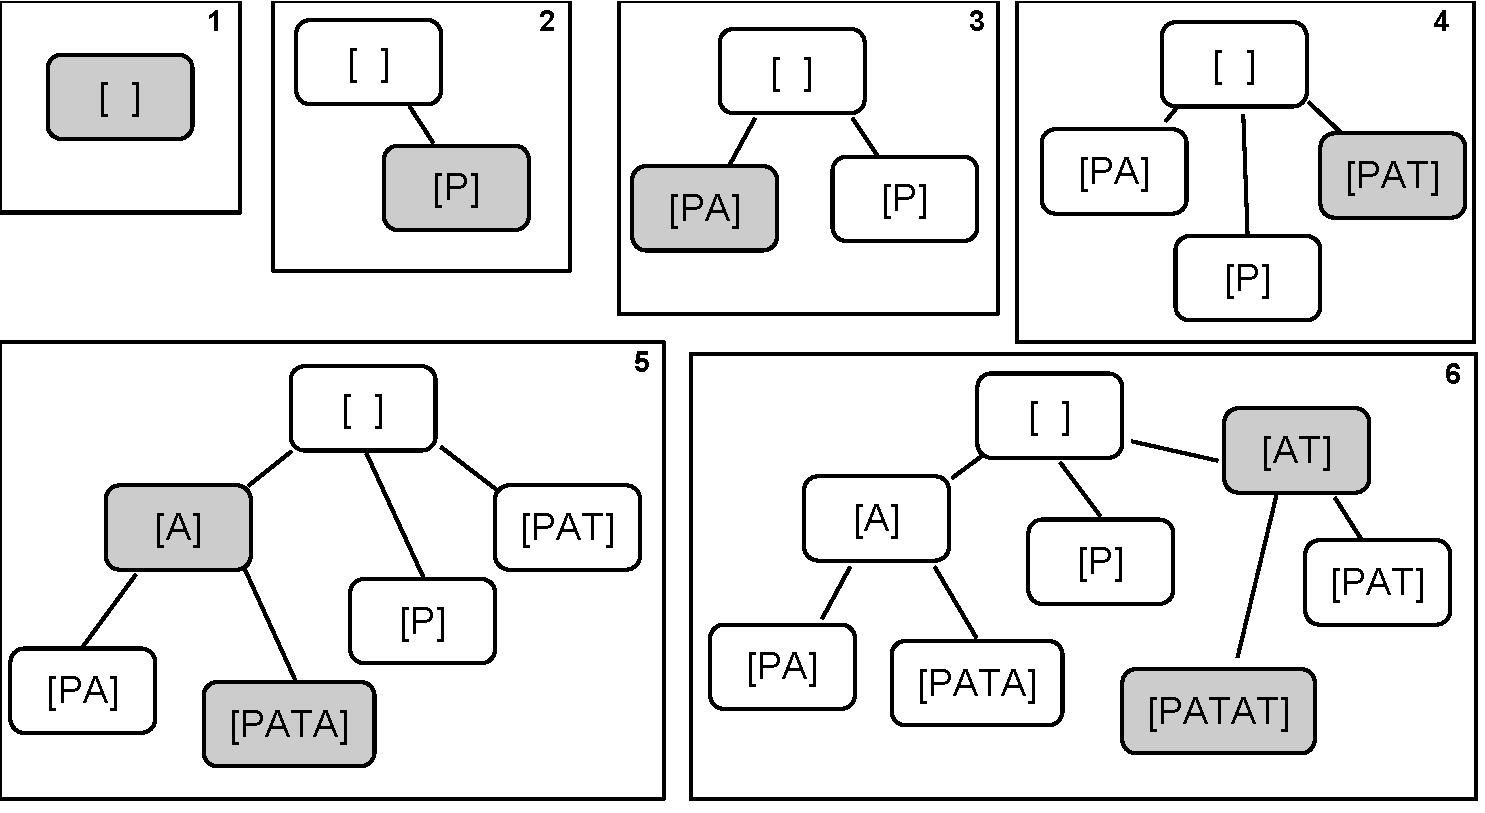
\includegraphics{figs/PATAT.pdf}} % [clip=true, viewport= 1in 1in 9in 9in]
%		\caption{Construction of suffix tree for string ``PATAT".  In each frame the new nodes are shaded in gray.}
%		\label{fig:suffix_tree}
%	\end{center} 
%\end{figure*} 
%

Our focus in this section is on providing the first comprehensive implementation reference for deplump with the changes necessary to achieve streaming asymptotics highlighted.  Many of the individual algorithms that appear in this section are justified and explained in detail in prior art.  We explain the functionality of each algorithm, but refer the interested reader to the prior art for detailed mathematical justifications, in particular \citep{Wood2009,Gasthaus2010,Bartlett2010}.

Given a sequence of symbols $\Seq = [s_0, s_1, s_2, \ldots]$ where each symbol $s_n$ comes from from an ordered set of symbols $\{\sigma_1, \sigma_2, \ldots\} = \Sigma$,  streaming deplump works by repeatedly producing a predictive distribution for the continuation of the sequence given the full preceding context and encoding the next symbol by passing that predictive distribution to an entropy encoder.  In this paper explicit details related to encoding and decoding are not included, instead we present the algorithms necessary to incrementally construct the predictive distributions needed by the encoder and decoder.  Specifically, we assume that if the predictive distribution function is $F$ and the next symbol in the stream is $s$ then the stream can be compressed using an entropy encoder that takes $F(s-1)$ and $F(s)$ as arguments and returns a bit stream (possibly null) \citep{Witten1987}.   The cumulative distribution function is well defined because the symbols are ordered. We use the notation $s-1$ to refer to the symbol prior to $s$ in the symbol set $\Sigma$.  %Note that the symbol set can be ordered as the set is discovered.
%Further, although there is a beautiful interplay between the algorithms presented herein and approximate inference in the underlying model, we have decided to, given the availability of referenced work on 
\begin{figure*}[ttt!]
	\begin{minipage}[t]{.48\linewidth}
		\begin{algorithm}[H]
			\caption{PMFNext} \label{alg:pmfnextsymbol}
	\begin{algorithmic}[1]
	\Function{$\{ \pi, \N \} \la $ PMFNext}{$\RS$}
		\While{$ |\RS| \geq T$}
%			\State Delete nodes referencing \RS[1] and update $nc$
			\State $\RS \la \sigma(\RS)$
		\EndWhile
		\While{ $\nc > (L - 2)$}
			\State Delete random leaf node
			\State $nc \la nc -1$
		\EndWhile
		
		\State $\N \la$ \textsc{GetNode}$(\RS, \T)$
		\State $\pi \la$ \textsc{PMF}($\N, \vec 0, 1.0$) \Comment{$| \vec 0| = | \Sigma|$}
	%	\State UpdateCountsAndDiscountGradients($\N,s,\pi_s,$TRUE)
%		\State \Return [$\pi$, \N]
	\EndFunction
	 \end{algorithmic}
\end{algorithm}
\vspace{-.75cm}
\begin{algorithm}[H]
	\caption{DrawCRP} \label{alg:drawcrp}
	\begin{algorithmic}[1]

	\Function{$t \la $ DrawCRP}{$n,d,c$} %\Comment{$ n \geq 1$}
		\State $t \la 1$
		\For{i = 2 : n}
			\State $r \la 0$
			\State $r  \la 1$ w.p. $\frac{td + c}{i-1 + c}$
			\State $t \la t + r$
		\EndFor
%		\State \Return $t$
	\EndFunction
	
	\end{algorithmic}	
\end{algorithm}
	 \end{minipage}
	\hfill
%
%
%%\begin{algorithm}
%	\caption{GetDiscount} \label{alg:getdiscount}
%    \begin{algorithmic}[1]
%    	\Function{PointOnCDFNextSymbol}{$h,\T,\RS$}
%		\While{$ |\RS| \geq 100 L$}
%			\State Delete nodes referencing \RS[0]
%			\State $\RS \la \sigma(\RS)$
%		\EndWhile
%		\While{ $\nc > (L - 2)$}
%			\State Delete leaf node uniformly at random
%		\EndWhile
%		\State $\N \la$ GetNode$(\RS, \T)$
%		\State $\pi \la$ PMF($\N, \vec 0, 1.0$) \Comment{$| \vec 0| = | \Sigma|$}
%		
%		\State $F(s) \la 0$
%		\State $s \la 0$
%		\While{$F(s) < h$}
%			\State $s \la s + 1$
%			\State $F(s) \la F(s) + \pi_s$
%		\EndWhile
%		
%		\State $F(s-1) \la F(s) - \pi_s$
%		\State Update $h$
%		\Return  $[h,s, F(s-1), F(s)]$
%	\EndFunction	
%	\Function{GetDiscount}{\N}
%		\State $d = 1.0$
%		\If{\N = [ ]}
%			\State \Return $\dd_0$
%		\EndIf
%		\For{$i = (|$\textsc{PA}$(\N)| + 1): |\N|$}
%			\If{$i \leq 10$}
%				\State $d \la d \delta_i$ \Comment{multiply by discount parameter $i$}
%			\Else
%				\State $d \la d \dd_{10}^{\alpha^i}$
%			\EndIf
%		\EndFor
%		\State \Return $d$
%	\EndFunction
%	
%		\end{algorithmic}
%\end{algorithm}
	\begin{minipage}[t]{.48\linewidth}
\begin{algorithm}[H]
	\caption{GetNode} \label{alg:getnode}
	\begin{algorithmic}[1]
    	\Function{$\Seq \la $ GetNode}{\Seq, \T}
		\State Find the node \M \space in the tree sharing the longest suffix with \Seq
		\If{\M \space is a suffix of \Seq}
%			\If{$\Seq = \M$ or $|\M| = D$}
%				\State \Return \M
			\If{$\Seq \neq \M$ and $|\M| <  D$}
				\State $\Seq \la$ \textsc{CreateNode}$(\Seq, \M)$
				\State $nc \la nc + 1$
%				\State \Return \Seq
			\EndIf
		\Else
			\State \PP \la \space \textsc{FragmentNode}(\M, \Seq)
			\State $\Seq \la $ \textsc{CreateNode}$(\Seq, \PP)$
			\State $nc \la nc + 1$
%			\State \Return \Seq
		\EndIf
	\EndFunction
	\end{algorithmic}	
\end{algorithm}
	\end{minipage}
	\end{figure*}

The algorithms of deplump run over a constant space, incrementally constructed suffix-tree-like data structure.  Note that the fact that this datastructure is of constant size is a significant point of  differentiation between this work and that of \cite{Gasthaus2010}. This tree-shaped data structure efficiently encodes a subset of the set of unique suffixes of all contexts in a sequence.  Each edge in the tree has a label which is a subsequence of the input sequence.  Each edge label is represented by two indices into a fixed-length suffix of the input sequence which we call the reference sequence (i.e.~each edge label is $[r_{i+1}, r_{i+2}, \ldots,r_{j}]$ for indices $i$ and $j$ into the reference sequence where $[r_{1} = s_{n-T}, \ldots, r_T = s_n]$ after every $n$th input sequence element is processed.)  
Therefore, each node in the tree corresponds to a subsequence $[s_m, \ldots, s_{m + k}]$ of the input sequence and a (potentially non-sequential) set of subsequences of the reference sequence.  
%The suffix a node corresponds to is determined by concatenating the edge labels on the path from the root to the node. (i.e.~the set $\{ [ ], [s_0], [s_0,s_1], [s_0, s_1,s_2], \ldots \}$)
We use $\N$ to refer interchangeably to a node and the suffix in the input sequence to which the node corresponds.  Note that for a given suffix the corresponding node is accessed by traversing edges of the tree that match the suffix read from right to left. 
\begin{algorithm}[t!]
	\caption{UpdateCountsAndDiscountGradients} \label{alg:updatecountsandgradients}
	\begin{algorithmic}[1]
	
	\Function{UpdateCountsAndDiscountGradients}{$\N, s, p$, BackOff}
	%	\State $d \la $ \textsc{GetDiscount}(\N)
		\State $pp \la p$
		\If{$c^\N > 0$}
			\State $pp \la (p - \frac{c^\N_s - t^\N_s d^{\N}}{c^\N})(\frac{c_\N}{t^\N d^{\N}})$
			\State $w \la c^\N_s	+ d^\N (t^\N pp   - t^\N_s)$		
		\EndIf
		
		\If{BackOff  and $c > 0$}
			\State $c^\N_s \la c^\N_s + 1$
			\State BackOff $\la 0$
			\State BackOff $\la 1$ w.p. $pp (\frac{t^\N d^{\N}}{w})$ \Comment{w.p abbreviates ``with probability"}
			\If{BackOff}
				\State $t^\N_s \la t^\N_s + 1$
			 \EndIf
		\ElsIf{BackOff}
				\State $c^\N_s \la c^\N_s + 1$;  $t^\N_s \la t^\N_s + 1$
		\EndIf
		
		\State \textsc{UpdateDiscountParameterGradients}%($t^\N_s, t^\N,pp, d^{\N}$)
		\State \textsc{UpdateCountsAndDiscountGradients}(\textsc{PA}(\N), $s,pp$, BackOff)
		\State \textsc{ThinCounts}(\N)
	\EndFunction
		\end{algorithmic}
\end{algorithm}

Streaming deplump is given in Algorithm~\ref{alg:deplump/plump}.  Deplump processes each element of an input sequence $\IS$ incrementally.  For each element $s_n$ of $\IS$, \textsc{PMFNext} computes the predictive probability mass function $\pi$ (conditioned on the observed context $[s_0, s_1, \ldots, s_{n-1}] = \RS$) needed for compression.  The element $s_n$ is then encoded by an entropy encoder with parameter $\pi$.  \textsc{PMFNext} also handles the incremental maintenance of the underlying constant-space datastructures by restricting the length of the reference sequence and by both constructing and deleting nodes in the tree as needed.  The final steps in streaming deplump are to incrementally integrate the observation into the approximated sequence memoizer and to adjust the back-off/smoothing parameters $\D$.  This involves updating counts in the tree and calculating a stochastic gradient for $\D$.  Both of these are done in \textsc{UpdateCountsAndDiscountGradients}. %The discount parameters are updated based on a learning rate $\eta$ and the encoded symbol in appended to $\RS$. 
The organization of functions in this way minimizes the number of tree traversals that need to be performed, tree traversals being a major component of the computational cost of this algorithm.

\textsc{PMFNext} (Alg.~\ref{alg:pmfnextsymbol}) starts by enforcing the bounds on $|\RS|$ and $|\mathcal{H}|$.  Both of these bounds require nodes to be removed from the tree (the first implicitly as a result of edge labels becoming undefined and the second explicitly).  Removing nodes from the underlying sequence datastructure has no consequence in and of itself, but as an operation on the corresponding sequence memoizer graphical model some care must be taken because node removal has ramifications in terms of what kinds of approximations are being imposed on inference.  \cite{Bartlett2010} showed that removing leaf nodes from the sequence memoizer results in a coherent approximate inference algorithm for the sequence memoizer.  So, enforcing the bound on $| \mathcal{H} | < L$ can be as simple as incrementally removing leaf nodes uniformly at random.  To facilitate random deletion we maintain a count in each node of the number of leaf nodes in the subtree below it.  A random leaf node can then be obtained by traversing a weighted random path down the tree.  

\begin{figure*}[ttt!]
\begin{minipage}[t]{.48\linewidth}
\begin{algorithm}[H]
	\caption{ThinCounts} \label{alg:thincounts}
	\begin{algorithmic}[1]
			
	\Function{ThinCounts}{$\N$}
	%	\State $d \la$ \textsc{GetDiscount}$(\N)$
		\While{$c^\N > k$}
			\State $\pi = [\frac{c^\N_{\sigma_1}}{c^\N}, \frac{c^\N_{\sigma_2}}{c^\N}, \ldots, \frac{c^\N_{\sigma_{|\Sigma}}}{c^\N}]$
			\State $s \la $ \textsc{Multinomial}$(\pi)$ %s.t. $\pi_l = \frac{c_l}{c}$ % \Comment{$\pi$ is a distribution over $\Sigma$}
			\State $\phi \la$ \textsc{Partition}$(c^\N_s, t^\N_s, d^{\N})$
			\State $\psi \la (\frac{1}{c^\N_{s}} ) \phi$
			\State $i \la$ \textsc{Multinomial}$(\psi)$
			\If{$\phi_i = 1$}
				\State $t^\N_s \la t^\N_s - 1$
			\EndIf
			\State $c^\N_s \la c^\N_s - 1$
		\EndWhile
	\EndFunction	
	
	\end{algorithmic}	
\end{algorithm}
\end{minipage}
\hfill
\begin{minipage}[t]{.48\linewidth}
\begin{algorithm}[H]
	\caption{PMF} \label{alg:pmf}
	\begin{algorithmic}[1]

	\Function{$\pi \la $ PMF}{$\N, \pi, m$}
%		\State $d \la $ \textsc{GetDiscount}(\N)		
		\If{$c^\N > 0$}
			\For{$\sigma \in \Sigma$}
				\State $\pi_\sigma\la \pi_\sigma + m(\frac{c^\N_\sigma - t^\N_\sigma d^{\N}}{c^\N})$
			\EndFor
		\EndIf
		
		\If{\textsc{PA}$(\N) \neq$ null}
			\State $\pi \la $ \textsc{PMF}(\textsc{PA}(\N), $\pi, d^{\N} m$)
		\Else
			\State $\pi \la (1- d^{\N} m)\pi + d^{\N}m\mathcal{U}_{\Sigma}$ %\Comment{$\mathcal{U}(\Sigma)$ is the uniform distribution over $\Sigma$}
%			\State \Return $\pi$
		\EndIf 
	\EndFunction
		\end{algorithmic}
\end{algorithm}
\end{minipage}
\end{figure*}

The removal of nodes due to their edge labels becoming undefined is an unfortunate consequence of having to constrain the reference sequence $\RS$ to be of constant length.  Note that without a bound $|\RS|$ would grow in length by one as each symbol of the input sequence is incorporated into the model.  To maintain the upper bound on $|\RS|$ we shorten $\RS$ by one as in a fixed length FIFO queue. Since the labels of edges in the tree index into $\RS$ then, when it is shortened, some edges may end up having labels that index beyond the retained elements of $\RS$ resulting in ``undefined'' edges.  Nodes below any undefined edges in the tree must be removed because they can no longer be accessed.  Their removal is justified in the same way as before because all subtree removals can be implemented as a cascade of leaf node removals.  It is desirable to minimize the number of nodes removed due to the incessant shortening of $\RS$.  One way to do this is to always update all edge indices on all paths traversed in the process of inserting nodes into the tree (that we do this is not made explicit in Alg.~\ref{alg:getnode} but on line 2 this updating of the edge indices should be performed)   \textsc{PMFNext} finishes by accessing the correct node for prediction using \textsc{GetNode} (Alg.~\ref{alg:getnode}) and the predictive probability mass function is calculated recursively by \textsc{PMF} (Alg.~\ref{alg:pmf}).

\begin{algorithm}[t!]
	\caption{FragmentNode} \label{alg:fragmentnode}
	\begin{algorithmic}[1]

	
	\Function{$\PP \la $ FragmentNode}{$\M, \Seq$}
%		\State $d^\M \la$ \textsc{GetDiscount}(\M)
		\State $\PP \la$ maximum overlapping suffix  of \M \space and \Seq
		\State $\PP \la $ \textsc{CreateNode}$(\PP,$ \textsc{PA}$(\M))$
		\State $nc \la nc + 1$
		\State\textsc{ PA}(\M) $\la \PP$
%		\State $d^\PP \la$ \textsc{GetDiscount}(\PP)
		\For{$\sigma \in \Sigma$}
			\State $\phi \la$ \textsc{Partition} $(c^\M_\sigma, t^\M_\sigma,d^\M)$
			\State $t^\PP_\sigma \la t^\M_\sigma$;  $t^\M_\sigma \la 0$
			\For{$i= 1 : | \phi|$}
				\State $a \la$ \textsc{DrawCRP}$(\phi[i],d^\M / d^\PP,-d^\M)$
				\State $t_\sigma^\M \la t_\sigma^\M + a$
			\EndFor
			\State $c^\PP_\sigma \la t^\M_\sigma$
		\EndFor
%		\State \Return \PP
	\EndFunction
		\end{algorithmic}
\end{algorithm}

Incremental construction of the tree is handled by the function \textsc{GetNode} within \textsc{PMFNext} which creates two or fewer nodes in the tree for every call.  Within the function \textsc{GetNode}, nodes are created by \textsc{CreateNode} and \textsc{FragmentNode}. The function \textsc{CreateNode(\N,\M)} simply creates a node $\N$ with parent $\M$. \textsc{FragmentNode} (Alg.~\ref{alg:fragmentnode}) implements the fragmentation operation developed in \citep{Wood2009} required to ensure proper sequence memoizer inference in the case where an edge must be split and a node inserted, but does so in the constant space node representation given in \citep{Gasthaus2011}.  This new intervening node corresponds to a predictive context and the counts corresponding to a proper estimate of this predictive distribution must be inferred.   Practically this means that value must be assigned to all counts $t_s^\mathcal{P}, c_s^\mathcal{P}, t_s^\mathcal{M}, c_s^\mathcal{M}$ for $s\in\Sigma$.  \textsc{FragmentNode} uses two functions to do this: \textsc{Partition}$(c,t,d)$ (Alg.~\ref{alg:samplepartition}) and \textsc{DrawCRP}$(n,d,c)$ (Alg.~\ref{alg:drawcrp}).  The net effect of \textsc{FragmentNode} is to create a new branching node at the shared suffix of $\mathcal{M}$ and $\mathcal{S}.$   The mathematical explanation of these algorithms is given in \citep{Gasthaus2011}.  % together implement the node fragmentation algorithm for the constant space node representation of the sequence memoizer discussed in \citep{Gasthaus2011}.% (this samples a partition following the $\mathcal{E}\mathcal{S}_{c}(d,0)$\footnote{ The two parameter Ewen's $\mathcal{E}\mathcal{S}_{n}(d,c)$ distribution is a distribution over partitions of $n$ objects and plays a key role in inference in models using Pitman-Yor distributions \cite{Ewens_dist_ref}.} distribution conditioned on the length of the partition being $t$).\textsc{DrawCRP}$(n,d,c)$ returns the length of a random partition drawn from the $\mathcal{E}\mathcal{S}_{n}(d,c)$.  %and is called when none of the existing tree nodes are a suffix of the context \RS.  
%An illustration of the incremental construction of a suffix tree can be seen in Figure~\ref{fig:suffix_tree} for the toy sequence [PATAT].  We use \textsc{PA}(\N) to refer to the parent of $\N$ in the tree.  In frame 4 the function \textsc{GetNode} assigns [ ]  to $\M$ and then [PAT] to $\Seq$ with $\M = \textsc{PA}(\Seq)$. In Frame 5 \textsc{GetNode} assigns [PA] to $\M$, but then must assign [A] = \textsc{FragmentNode}(\M) to $\PP$ and \textsc{PA}$(\M)$ to \PP.  Node $\Seq$ is then created by \textsc{CreateNode}$($[PATA]$,\PP)$.   % In each frame the first step is to find $\M$, which can be achieved by descending an appropriate path of the suffix tree.  All of the nodes on the path to $\M$ and possibly $\M$ itself can have the indices into $\RS$ updated to point to a more recent section of the reference sequence. 

\begin{algorithm}[t!]
	\caption{Partition} \label{alg:samplepartition}
	\begin{algorithmic}[1]
	
	\Function{$\phi \la  $ Partition}{$c,t,d$}
		\State $M \la  t \times c$ matrix of zeros
		\State $M(t,c) \la 1.0$
		\For{$j = (c-1) : 1$}
			\For{$i = 1 : (t-1)$} 
				\State $M(i,j) \la M(i +1, j+1) + M(i,j+1)(j - id)$ 
			\EndFor
			\State $M(d,j) \la M(t,j+1)$
		\EndFor
		\State $\phi \la [1,0,0,\ldots, 0]$ \Comment{$|\phi| = t$}
		
%		\State $\phi \la \vec 0$ \Comment{$|\vec 0| = t$}
	%	\State $\phi[1] \la 1$;  $k \la 1$
		\For{j = 2 : c}
			\State $M(k,j) \la M(k,j)(j-1 -k d)$
			\State $r \la 0$
			\State $r \la 1 $ w.p. $\frac{M(k+1,j)}{M(k+1,j) + M(k,j)}$
			\If{r = 1}
				\State $k \la k + 1$
				\State $\phi[k]  \la 1$
			\Else
				\State $i \la$ \textsc{Multinomial}$([\frac{\phi[1] - d}{j-1 -kd}, \frac{\phi[2] - d}{j-1 -kd}, \ldots, \frac{\phi[k] - d}{j-1 -kd}])$
				\State $\phi[i] \la \phi[i] + 1$
			\EndIf
		\EndFor
%		\State \Return $\phi$
	\EndFunction
		\end{algorithmic}
\end{algorithm}

Finally \textsc{UpdateCountsAndDiscounts} (Alg.~\ref{alg:updatecountsandgradients}) integrates the observation into the underlying probability model, adjusting counts in potentially all nodes on the path from the context in which the observation was made to the root of the context tree.   \textsc{UpdateCountsAndDiscounts} also computes a partial stochastic gradient for the discount parameter of each node on this path (this gradient is used in \textsc{Deplump} to update $\mathcal{D}$).  The details of the discount computation performed in \textsc{UpdateDiscountParameterGradients} are too long to include but can be obtained from \cite{Gasthaus2010}.  \textsc{UpdateCountsAndDiscounts} also uses \textsc{ThinCounts} (Alg.~\ref{alg:thincounts}) to enforce the bound on the counts in each node required to ensure computational asymptotics appropriate for streaming compression. 


%Each node instance $\N$ contains two counts for each $\sigma \in \Sigma$, $c_\sigma$ and $t_\sigma$.  We use $c$ and $t$ to refer to the marginal counts $\sum_{\sigma \in \Sigma} c_\sigma$ and $\sum_{\sigma \in \Sigma} t_\sigma$.  Each node also has a discount associated with it which we refer to as $d^\N$ in the algorithms. If we define $\delta_{n} = \delta_{10}^{\alpha^{n - 10}}$ for $n \geq 10$ then $d^{\N} = \Pi_{i =|\textsc{PA}(\N)| + 1}^{|\N|} \delta_{i}$ if $\N$ is not the root and $\delta_{0}$ if $\N$ is the root.  Counts are updated and discount parameter gradients are calculated by Algorithm~\ref{alg:updatecountsandgradients}.  The new approximation discussed in Section~\ref{section:methodology} is implemented by \textsc{ThinCounts}.

%The reference sequence grows with the length of the input sequence and must be shortened as the algorithm progresses.  When $\RS$ is shortened, nodes in the suffix tree which reference removed sections are no longer usable and must be removed from the tree to prevent a memory leak.  To facilitate the removal process pointers are maintained from the elements of $\RS$ to the suffix tree nodes which reference them.  Without the use of pointers, deletion of the unusable nodes requires a search over the tree which is prohibitive for large trees. The cost of these operations can be amortized by shorting $\RS$ in chunks and keeping pointers from each chunk of $\RS$ instead of each element.  

%The reference sequence $\RS$ is implemented as a linked list. Therefore, instead of using a simple $i,j$ index in each suffix tree node, $i$ is replaced by a linked list node and an offset and $j$ is replaced by a string length $l$.  Each node of the linked list must contain a list of suffix tree nodes which reference it.  The reference sequence grows as the length of the input sequence grows and must be shortened as the algorithm progresses.  The shortening of $\RS$ is made explicit by the $\sigma$ operator in CDFNextSymbol, which returns the argument sequence shortened by removing the fist element.  When $\RS$ is shortened, nodes in the suffix tree which reference removed sections are no longer usable and must be removed from the tree to prevent a memory leak.  Without a list of suffix tree nodes which reference each linked list node, deletion of the unusable nodes requires a search over the tree which is prohibitive for large trees.  The cost of these operations can be amortized by shorting $\RS$ in chunks, i.e. by removing nodes of the linked list.  To minimize the impact of rendering nodes unusable by shortening the reference sequence, nodes should be updated to point to the most recent part of $\RS$ as possible.

%The function \textsc{Multinomial} is used in several of the algorithms and returns a single value sampled from a discrete distribution.   The  distribution shows up here in the functions \textsc{DrawCRP(n,d,c)}, which is called in \textsc{FragmentNode}, \textsc{Partition}.   \textsc{DrawCRP(n,d,c)} returns the length of a random partition drawn from the $\mathcal{E}\mathcal{S}_{n}(d,c)$.  The function \textsc{Partition(c,t,d)} implements the seating arrangement reconstruction algorithm discussed in \citep{Gasthaus2011} to sample a partition following the $\mathcal{E}\mathcal{S}_{c}(d,0)$ distribution conditioned that the length of the partition be $t$.

To use streaming deplump a choice of approximation  parameters must be made.  The full set of these parameters consists of $\D$, $D$, $T$, $k$, $L$, $\eta$.  $\D = [\dd_0, \dd_1, \ldots, \dd_{10}, \alpha]$ is a list of discount parameters, each taking a real value in $(0,1)$.  $D$ is the maximum depth of the suffix tree which corresponds to both the maximum context length used in modeling and the maximum recursion depth of all of the algorithms.  $T$ is the bound on the length of the reference sequence $\RS$ and is typically set to a multiple of the upper bound on the number of node instances in the suffix tree $L$.  The parameter $k$ is the upper bound on the total count $c^\N$ in each node.  The parameter $\eta$ is a learning rate for the updating of the discount parameters and is typically set to a very small value.  

%For each $s$ in the input sequence the function \textsc{PMFNextSymbo}l is called to obtain the predictive probability mass function (PMF).  After encoding or decoding using the predictive PMF $pi$ the first step in updating the model estimate is performed by the function \textsc{UpdateCountsAndDiscounts}.  Starting at node $\N$ and progressing up to the root of the tree, $c_s$ is incremented if $t_s$ was incremented in the node below.  If $c_s$ is incremented, a stochastic decision is made to increment $t_s$.  The gradients for the discount parameters $\D$ are updated by the function \textsc{UpdateDiscountParameterGradients}.  If $c$ is larger than $k$ in any of the nodes, the counts $c_s$ and potentially $t_s$ are reduced by the function \textsc{ThinCounts}. Finally, \D \space is updated based on the calculated gradients and the specified learning rate $\eta$ and the symbol is appended to \RS.





%\begin{algorithm}
%	\caption{UpdateDiscountParameterGradients} \label{alg:updatediscountparametergradients}
%	\begin{algorithmic}[1]
%
%
%	\Function{UpdateDiscountParameterGradients}{$\N, t_s, c, t, pp, d, m$}
%		\If{$c > 0$}
%			\If{$|\N| = 0$}
%				\State $ \psi \la \frac{1.0}{\dd_0}$
%				\State $\G_0 \la \G_0 + (d(t * pp - t_s)\psi / c)  m$
%			\Else
%				\State $z \la |$\textsc{PA}(\N)$| + 1$
%				\While{$z \leq |\N|$ and $z < 10$}
%					\State $\psi \la \frac{1.0}{\dd_z}$
%					\State $\G_z \la \G_z + (d(t * pp - t_s) \psi / c)  m$	
%				\EndWhile
%				
%				\If{$|\N| \geq 10$}
%					\State $a \la z - 10$
%					\State $b \la |\N| - z + 1$
%					\State $\psi \la \alpha^a(1 - \alpha^b) / ((1 - \alpha)  \dd_{10})$ 
%					\State $\G_{10} \la \G_{10} + (d(t * pp - t_s) \psi / c)  m$	
%					\State $\psi \la$ log$(\dd_{10}) (a \alpha^{a-1} - (a + b)\alpha^{a + b-1}) / (1 - \alpha) + (\alpha^a - \alpha^{a + b}) / (1 - \alpha)^2$
%					\State $\G_{11} \la \G_{11} + (d(t * pp - t_s)\psi / c)  m$	
%				\EndIf
%			\EndIf
%		\EndIf
%	\EndFunction
%
%	\end{algorithmic}	
%\end{algorithm}

% !TEX root = deplump.tex
\section{Experiments}
\label{sec:experiments}

As the performance of batch deplump was established relative to other lossless compressors for a variety of datatypes in \citep{Gasthaus2010}, we focus our experiments on establishing a) that the approximations to inference in the sequence memoizer combined in this paper in order to make deplump a streaming compressor do not significantly adversely affect compression performance, b) that the resulting compressor can indeed compress extremely long sequences as the asymptotic guarantees would suggest it should, and c) what settings of the approximation parameters produce the best compression performance.

Before testing the algorithm on streaming corpus we compared the algorithm to batch deplump.  We compressed the 100Mb Wikipedia corpus used for the Hutter Prize \citep{Hutter2006} using the streaming variant of deplump with $L = 10^{7}$ and $D = 16$ and found it gives a compression ratio of 4.78.  Using batch deplump gives a compression ratio of 4.82 \citep{Gasthaus2010}, while running batch deplump repeatedly on the 5Mb subsections of the corpus reduces the compression ratio to 4.25.  These results demonstrate that the approximations made for streaming deplump give it a significant advantage over compressing the file in chunks and have very little negative effect when compared to the full model.

All of the experiments included in this paper use a complete Wikipedia text content dump \citep{Wikipedia} as a test corpus (26.8Gb uncompressed, 7.8Gb gziped and ??Gb paq9a'ed, each with default parameters, and 3.9Gb deplumped).  To establish what approximation parameters produce the best compression results we first ran streaming deplump on the first 100Mb section of the corpus limiting the depth to two different values ($D=16$ and $D=1024$) with a fixed limit on the number of nodes in the tree ($L=10^6$).  We observed that in both cases only very few nodes had high total counts ($c > 8,192$) suggesting that it might be possible to set the count upper bound to a relatively low value ($k= 8,192$) without significant compression performance degradation.  %That compression performance should not be affected by a reasonable count bound follows intuitively from the fact that in byte sequences $|\Sigma| = 256$ and setting $k=10,000$ is similar in effect to using 10,000 observations to estimate a 256 element discrete distribution.  
To ensure that compression performance did in fact not suffer, we compressed ten 100Mb subsections of the corpus (sampled randomly with replacement) for multiple values of $k$ between 128 and 32,768 (fixing $L=10^6$ and $D=16$).  We observed that average compression performance varied insignificantly over $k$ for $2^7 \leq k \leq s^{15}$.

 In each of the following experiments, subsections of the corpus were sampled with replacement.  In the first experiment the sampled subsections were all of size 100Mb, while in the second the sampled subsections varied in length.  In the first experiment, the interplay between limiting the number of nodes in the tree and restricting the depth of the tree was explored (results for which are shown in Figure~\ref{fig:varying_depths}).  Here $k$ was set to 8,192, while $L$ and the depth of the tree $D$ were varied as indicated in the figure.  In the second experiment, the interplay between stream length and node limit was explored (Figure~\ref{fig:varying_stream_length}).  In this experiment $k$ remained fixed at the same value and the depth was set to $D=16$ while $L$ varied as shown in the figure.  

Figure~\ref{fig:varying_depths} indicates that compression performance becomes essentially indistinguishable for depth restrictions greater than $D=10$.  However, this figure also suggests that compression performance almost always improves as a function of the number of nodes in the tree for depths 6 and greater.  Figure~\ref{fig:varying_stream_length} illustrates that the algorithm not only scales to very long sequences, but average compression performance continues to improve as the sequence grows.  Using a large value of $L$ appears to be beneficial for very long sequences.

\begin{figure*}[t] 
	\begin{center}
		\scalebox{.6}{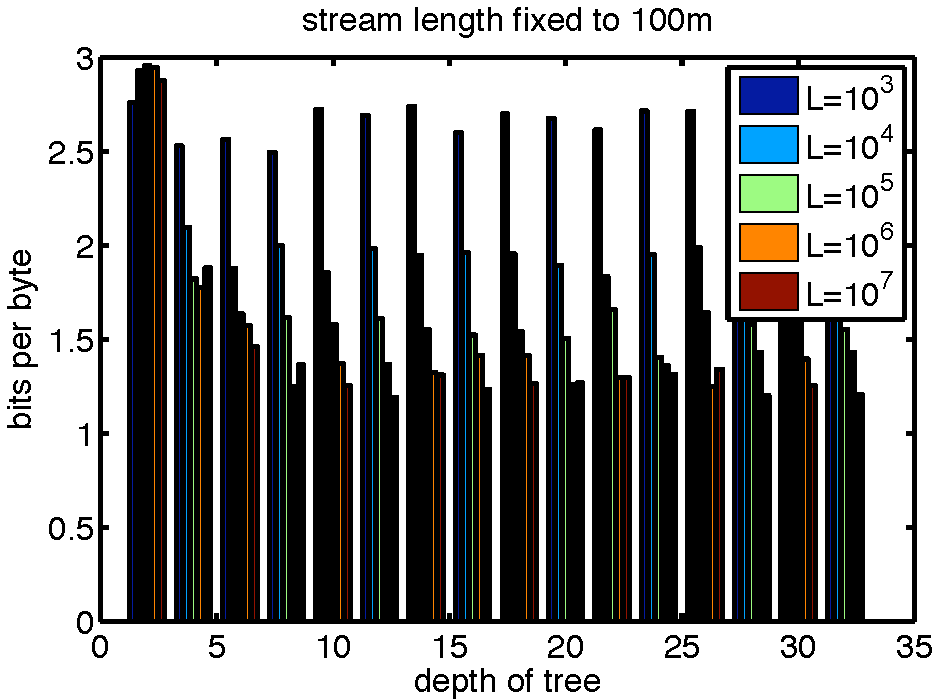
\includegraphics{figs/varying_depths.pdf}} % [clip=true, viewport= 1in 1in 9in 9in]
		\caption{Performance averaged over 10 random sections  100Mb sections of the corpus for varying fixed depths and number of allowable nodes ($L$) }
		\label{fig:varying_depths}
	\end{center} 
\end{figure*} 

%\begin{figure*}[t] 
%	\begin{center}
%		\scalebox{.6}{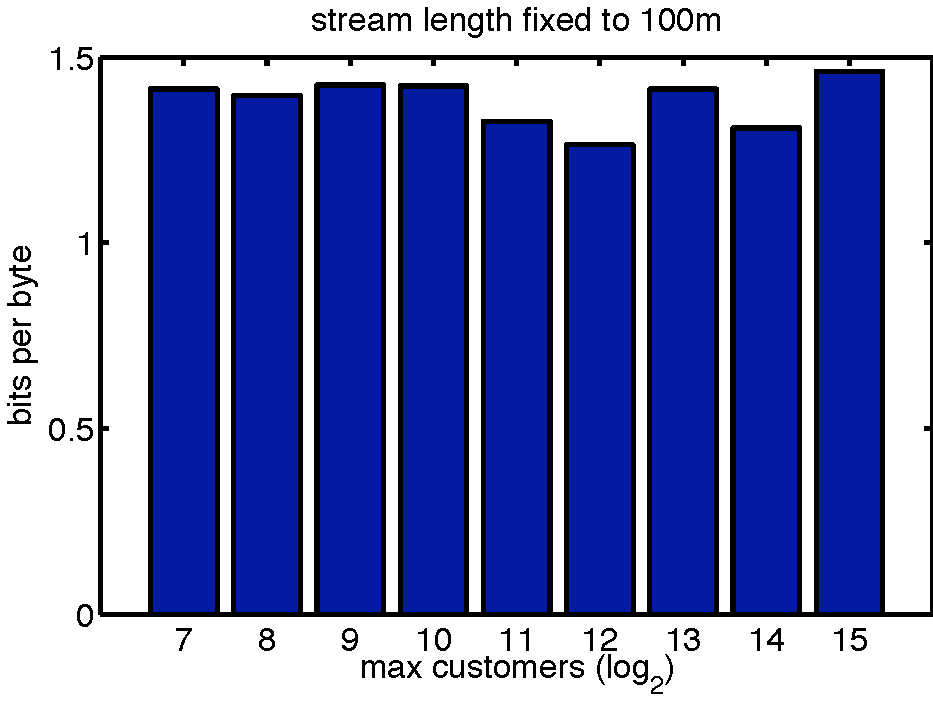
\includegraphics{figs/varying_max_customers.pdf}} % [clip=true, viewport= 1in 1in 9in 9in]
%		\caption{Performance for varying max allowable customers $k$.}
%		\label{fig: varying_max_customers}
%	\end{center} 
%\end{figure*} 

\begin{figure*}[t] 
	\begin{center}
		\scalebox{.6}{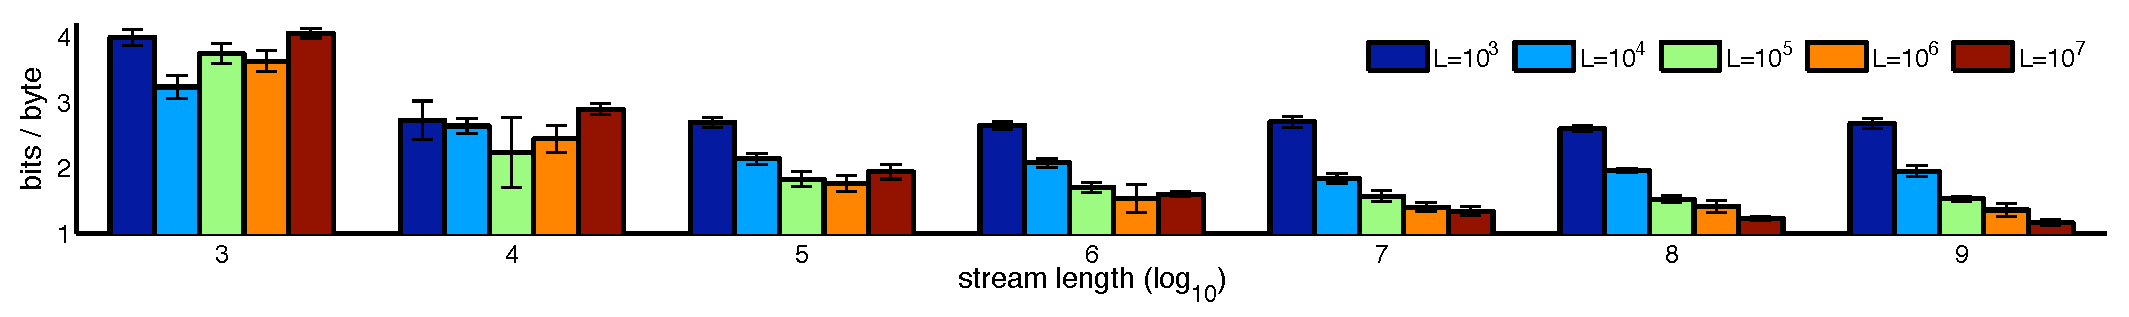
\includegraphics{figs/varying_stream_length.pdf}} % [clip=true, viewport= 1in 1in 9in 9in]
		\caption{Performance for varying stream lengths and number of allowable nodes ($L$).}
		\label{fig:varying_stream_length}
	\end{center} 
\end{figure*} 


%\begin{figure*}[t] 
%	\begin{center}
%		\scalebox{1}{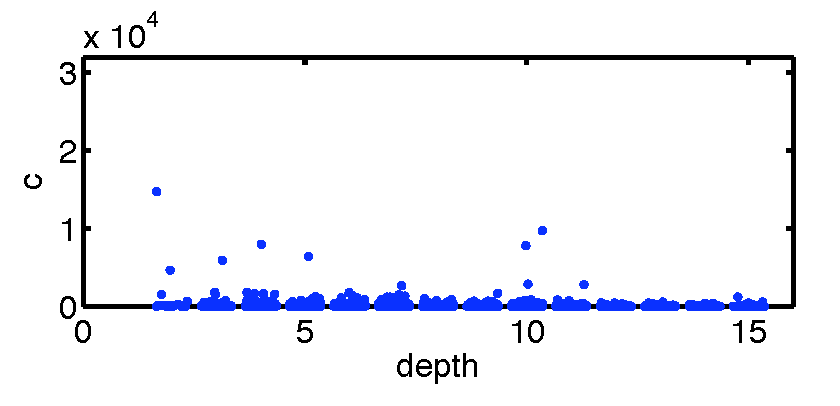
\includegraphics{figs/scatter_16.pdf}} % [clip=true, viewport= 1in 1in 9in 9in]
%		\caption{Scatter plots to explore the relationship between the depth of a node and the total count}
%		\label{fig:restaurant_plots}
%	\end{center} 
%\end{figure*} 

%\begin{figure*}[t] 
%	\begin{center}
%		\scalebox{1}{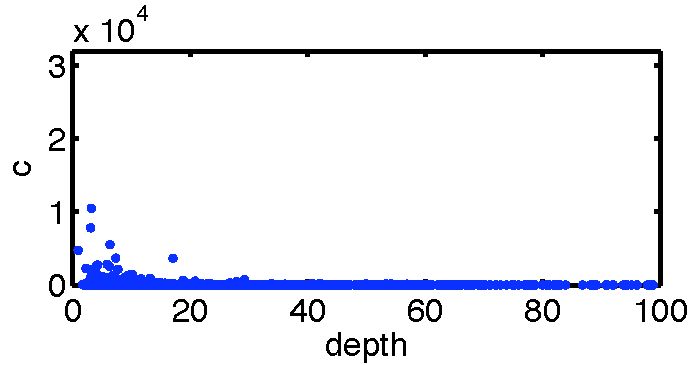
\includegraphics{figs/scatter_1024.pdf}} % [clip=true, viewport= 1in 1in 9in 9in]
%		\caption{Scatter plots to explore the relationship between the depth of a node and the total count}
%		\label{fig:restaurant_plots}
%	\end{center} 
%\end{figure*} 

% !TEX root = deplump.tex
\section{Conclusion}
\label{sec:conclusion}


%\section{Bayesian PDFA Inference}

The outline of this section is as follows.  We define a prior distribution over PDFAs with a fixed number of states and show that many of the parameters can be integrated out.  We derive a Metropolis-Hastings sampler for posterior inference in the finite model, and show that many of the elements of the transition matrix can be ignored without affecting the correctness of sampling.  We then let the number of states go to infinity and show that the limit is well defined.  This is the probabilistic deterministic infinite automaton (PDIA).  Inference in the PDIA carries over from the finite case in a natural way.

\subsection{A Prior over PDFAs}

We assume that the states $Q$, alphabet $\Sigma$ and initial state $q_0$ are known, and define a prior over the transition function $\delta$ and emission probabilities $\pi$.  In the finite case $\delta$ and $\pi$ can be thought of as matrices, with columns indexing elements of $\Sigma$ and rows indexing elements of $Q$.  For each column $j$ of the transition matrix $\delta$, we sample the rows i.i.d. from a discrete distribution $\bphi_j$ over $Q$, that is, $\delta \sim [\bphi_1\ldots\bphi_{|\Sigma|}]$.  The $\bphi_j$ themselves are sampled i.i.d. from a Dirichlet prior with parameters $\alpha\bmu$, where $\alpha$ is a concentration and $\bmu$ is itself drawn from a uniform Dirichlet distribution, with $\gamma$ total pseudocounts.  This hierarchical Dirichlet construction allows elements of $\delta$ to be coupled together in a way that remains well-behaved in the limit of infinite states.  We also place a uniform Dirichlet prior over the per-state emission probabilities $\bpi_i$ with $\beta$ total pseudocounts.  Formally:

\begin{eqnarray}
\bmu|\gamma,|Q| & \sim & \mathrm{Dir}\left(\gamma/|Q|,\ldots,\gamma/|Q|\right) \label{gen:mu} \\
\bphi_{j}|\alpha,\bmu  & \sim & \mathrm{Dir}(\alpha\bmu) \label{gen:phi} \\
\bpi_{i}|\beta,|\Sigma| & \sim & \mathrm{Dir}(\beta/|\Sigma|,\ldots,\beta/|\Sigma|) \label{gen:pi}\\
\delta_{ij} & \sim & \bphi_{j} \label{gen:delta}
\end{eqnarray}

where $i$ goes from 0 to $|Q|-1$ and $j$ goes from 1 to $|\Sigma|$.  From this we generate a sequence of $T$ symbols:

\begin{eqnarray}
\q_0 & = & q_0 \label{gen:q0} \\
x_0 & \sim & \bpi_0 \label{gen:x0} \\
\q_t & = & \delta(\q_{t-1},x_{t-1}) \label{gen:q} \\
x_t & \sim & \bpi_t \label{gen:x}
\end{eqnarray}

We choose this particular inductive bias, with transitions tied together within a column of $\delta$, because the most recent symbol ought to be informative about what the next state is.  If we instead had a single Dirichlet prior over all elements of $\delta$, transitions to a few states would be highly likely no matter the context and those states would dominate the behavior of the automata.  If we tied together rows of $\delta$ instead of columns, being in a particular state would tell us more about the sequence of states we came from than the symbols that got us there.  As we would like states to be good statistics of the past for predicting the future, a bias that depends on the most recent symbol is preferable.

Given data, the likelihood is

\[ p(x_{0:T}|\delta,\pi) = \pi(\q_0,x_0)\prod_{t=1}^T \pi(\q_t,x_t) \label{x:def} \]

We can marginalize out $\pi$ and express the likelihood in a form that depends only on the counts of symbols emitted from each state.  Define the count matrix $c$ for the sequence $x_{0:T}$ and transition matrix $\delta$ as $c_{ij} = \displaystyle\sum_{t=0}^T I_{ij}(\q_t,x_t)$, where $I_{ij}(\q_t,x_t)$ is an indicator function that is 1 if $\q_t = q_i$ and $x_t = \sigma_j$, 0 otherwise. This matrix gives the number of times each symbol is emitted from each state.  Thanks to multinomial-Dirichlet conjugacy we can integrate out $\pi$ and express the probability of a sequence given the transition function $\delta$ solely in terms of $c$ and $\beta$:

\begin{eqnarray}
 p(x_{0:T}|\delta,\beta) & = & \int p(x_{0:T}|\pi,\delta) p(\pi|\beta) d\pi \label{x:factor} \\
 & = &  \prod_{i=0}^{|Q|-1} \frac{\Gamma(\beta)}{\Gamma(\frac{\beta}{|\Sigma|})^{|\Sigma|}} \int\pi_{i1}^{\frac{\beta}{|\Sigma|}+c_{i1}-1} \pi_{i2}^{\frac{\beta}{|\Sigma|}+c_{i2}-1} \ldots \pi_{i|\Sigma|}^{\frac{\beta}{|\Sigma|}+c_{i|\Sigma|}-1} d\bpi_i \label{x:int}\\
 & = & \prod_{i=0}^{|Q|-1} \frac{\Gamma(\beta)}{\Gamma(\frac{\beta}{|\Sigma|})^{|\Sigma|}} \frac{\prod_{j=1}^{|\Sigma|}\Gamma(\frac{\beta}{|\Sigma|} + c_{ij})}{\Gamma(\beta + \sum_{j=1}^{|\Sigma|} c_{ij})} \label{x:end}
 \end{eqnarray}
 
 The dependence of $c$ on $\delta$ is only through $\q_{0:T}$, and changing a single element of $\delta$ can have a complex effect on $c$.  By changing a single transition $\delta_{ij}$, all states downstream of the first time $q_i$ emits $\sigma_j$ are affected, and some elements of $c$ that were zero may become nonzero, and vice versa.
 
 The likelihood of a particular transition matrix $\delta$ given $\bmu$ has a similar form.  Let $v_{ij}$ be the number of times that $\delta_{i'j} = q_i$ for all $i'$ in the column $j$, that is, $v_{ij} = \displaystyle\sum_{i' = 0}^{|Q|-1} I_{i}(\delta_{i'j})$, $I_i(q_{i'})$ being the indicator function that is only 1 when $q_i' = q_i$.  Given $\bmu$, we can integrate out $\phi$ and express the likelihood of $\delta$ in terms of $\bmu$:
 
 \begin{eqnarray}
 p(\delta|\bmu,\alpha) & = & \int p(\delta|\phi)p(\phi|\bmu,\alpha) d\phi \label{delta:factor}\\
  & = & \prod_{j=1}^{|\Sigma|} \frac{\Gamma(\alpha)}{\prod_{i=0}^{|Q|-1}\Gamma(\alpha\mu_i)} \int \phi_{0j}^{\alpha\mu_0+v_{0j}-1} \phi_{1j}^{\alpha\mu_1+v_{1j}-1} \ldots \phi_{|Q|-1,j}^{\alpha\mu_{|Q|-1}+v_{|Q|-1,j}-1} d\bphi_j \label{delta:int}\\
  & = &  \prod_{j=1}^{|\Sigma|} \frac{\Gamma(\alpha)}{\prod_{i=0}^{|Q|-1}\Gamma(\alpha\mu_i)} \frac{\prod_{i=0}^{|Q|-1} \Gamma(\alpha\mu_i + v_{ij})}{\Gamma(\alpha + |Q|)} \label{delta:end}
  \end{eqnarray}

%Finally, the posterior probability of $\bmu$ given $\delta$ is

%\begin{eqnarray}
%p(\bmu|\delta,\alpha, \gamma) & = & \frac{p(\delta|\bmu,\alpha)p(\bmu|\gamma)}{\int p(\delta|\bmu,\alpha)p(\bmu|\gamma) d\bmu}
%\end{eqnarray}

These are the ingredients we need for posterior inference.
 
 \subsection{Posterior Inference in the Finite Model}
 
We perform posterior inference in the finite model by Gibbs sampling elements of $\delta$ and the vector $\bmu$.  From the formulas above, it is straightforward to write down the conditional probability for one element of the transition matrix $\delta$.  If $\delta_{ij}$ is the element we are sampling, and $\delta_{-ij}$ is the rest of the matrix, with $\delta_{ij}$ removed, then

\begin{equation}
p(\delta_{ij}|\delta_{-ij},x_{0:T},\bmu,\alpha) \propto p(x_{0:T}|\delta_{ij},\delta_{-ij})p(\delta_{ij}|\delta_{-ij},\bmu,\alpha) \label{delta:cond}
\end{equation}

Both terms on the right hand side of this equation have closed-form expressions, the first given in \eqref{x:end}.  The second can be found from \eqref{delta:end} to be

\begin{equation}
P(\delta_{ij} = q_{i'}|\delta_{-ij},\alpha,\bmu) = \frac{\alpha\mu_{i'} + v_{i'j}}{\alpha + |Q| - 1} \label{delta:pred}
\end{equation}

Where $v_{i'j}$ is the number of elements in column $j$ equal to $q_{i'}$ {\em excluding} $\delta_{ij}$.  As $|Q|$ is finite, we can construct and normalize the conditional probability vector for $\delta_{ij}$ and sample.

We can simplify inference by ignoring transitions $\delta_{ij}$ for which the corresponding count $c_{ij}$ are 0.  Note that the likelihood of the data on the right hand side of \eqref{delta:cond} does not depend on $\delta_{ij}$ if $c_{ij} = 0$, so sampling conditioned on the data is the same as sampling without conditioning on the data.  Thus, if changing some other transition means $c_ij$ becomes 0, we can remove $\delta_{ij}$ until another transition is changed so the count again is nonzero, and we sample a new value for $\delta_{ij}$ from \eqref{delta:pred}, just as we would have during Gibbs sampling had we not removed it.  Note that the joint distribution over a column of $\delta$ is exchangeable, and so removing an observation is the same as marginalizing it out, meaning that sampling the other elements of $\delta$ is still correct, but now conditioned on the model where superfluous transitions are marginalized out.  When we remove multiple elements from a column of $\delta$, we have to replace the $|Q| - 1$ in the denominator of \eqref{delta:pred} with $K^+_j = \sum_{i=0}^{|Q|-1}v_{ij} \leq |Q|$, the number of entries in the $j$th column of $\delta$ that are {\em not} marginalized out.

The posterior for $\bmu$ up to a normalization constant is

\begin{eqnarray}
p(\bmu|\delta,\alpha,\gamma) & \propto & p(\bmu|\gamma) p(\delta|\bmu,\alpha)\nonumber \\
& = & \frac{\Gamma(\gamma)}{\Gamma(\frac{\gamma}{|Q|})^{|Q|}}(\mu_1\ldots\mu_{|Q|})^{\frac{\gamma}{|Q|}-1}\prod_{j=1}^{|\Sigma|} \frac{\Gamma(\alpha)}{\prod_{i=0}^{|Q|-1}\Gamma(\alpha\mu_i)} \frac{\prod_{i=0}^{|Q|-1} \Gamma(\alpha\mu_i + v_{ij})}{\Gamma(\alpha + K^+_j)}
\end{eqnarray}

We can sample this by Metropolis-Hastings, for example using Dir($\eta\hat\bmu$) as the proposal, where $\hat\bmu$ is our current estimate and $\eta$ is a large concentration parameter, or take the MAP estimate as in \cite{Mackay1995}.  Fortunately in the infinite limit a more natural way to sample presents itself.
 
 \subsection{The Probabilistic Deterministic Infinite Automaton}
 
 We now consider what happens when $|Q|\rightarrow\infty$.  Given a finite amount of data, there can only be nonzero counts for a finite number of state/symbol pairs, so we can marginalize out all but at most $T$ elements of $\delta$.  Denote these active entries by $\delta^T$.  The predictive probability for a new $\delta_{ij} = q_{i'}$ given $\delta^T$ is given by $\frac{\alpha\mu_{i'} + v_{i'j}}{\alpha + K^+_j}$.  Note that this only depends on $|Q|$ through $\mu_{i'}$, which is well behaved as $|Q|$ grows.  In the limiting case, most of the mass of $\bmu$ will concentrate on a handful of elements, and $\bmu$ becomes a draw from a {\em Dirichlet process} (DP), which is commonly used as a prior in Bayesian models with infinite parameters.  The hierarchical Dirichlet construction given in \eqref{gen:mu} and \eqref{gen:phi} becomes a {\em hierarchical Dirichlet process} (HDP), where the $\bphi_j$ are draws from a Dirichlet process whose parameters are given by $\alpha$ and $\bmu$, which is itself a draw from a Dirichlet process.  An attractive property of HDPs is that both the $\bphi_j$ and $\bmu$ can be integrated out, which makes sampling more straightforward than in the finite case.  This  representation of the model, with all draws from a DP integrated out, is known as the {\em Chinese Restaurant Franchise} (CRF).  This curious name needs some explanation, which we happily provide.
 
%We can sample incrementally from the joint distribution over $x_{0:T}$ and $\delta$ when $\phi_j$, $\mu$ and $\pi_i$ are integrated out in the $|Q|\rightarrow\infty$ limit.  From the start state $q_0$, we sample a symbol $s_{j_0}$ uniformly and assign $\delta_{0j_0}$ to a new state.  If $q^t = q_i$ then $x_t$ has the probability

% \[P(x_t=s_j|q_i,x_{0:t-1},q^{0:t-1}) = \frac{c_{ij}+\frac{\beta}{|\Sigma|}}{c_{i\cdot} + \beta}\]
 
% where $c_{ij}$ is the number of times so far $s_j$ was emitted from $q_i$ and $c_{i\cdot}$ is the total number of times $q_i$ has been visited so far.  
 
%If the state/symbol pair $(q_i,s_j)$ has not been visited before, we have to sample $\delta_{ij}$.  The two-stage generative procedure for elements of $\delta$ means that we have to keep track of counts at two levels.  Each $\delta_{ij}$ belongs to a cluster $v_{kj}$ that contains other $\delta_{i'j}$, while each $v_{kj}$ belongs to a top-level cluster $w_{l}$ that has elements across all $j$.  Each top level cluster has one $q \in Q$ assigned to it, and $\delta_{ij}$ is equal to that $q$ in the top cluster that the cluster with $\delta_{ij}$ belongs to (*might want to make this part clearer...add a figure*).  Let $\delta^t$ denote the elements of $\delta$ that have been visited at time $t$.  as follows:
 
%\[P(\delta_{ij} = k|\delta^t) \propto \begin{cases} & if $k \leq |\delta^t|$ \cr  & if $k > |\delta^t|$ \end{cases}\]
 
% This process for sampling from an HDP when $\mu$ and $\phi_j$ are integrated out is known as the {\em Chinese Restaurant Franchise Process}.

% \section{Posterior Inference over PDFAs}
 
 We perform posterior inference by sampling assignments for $\delta_{ij}$ individually.  Rather than ordinary Gibbs sampling, we use a mixed Gibbs/Metropolis-Hastings update.  To see why, consider the following case:  $\delta_{ij}$ is the only sampled element of $\delta$ that is assigned to the state $q_{i'}$.  When we removed $\delta_{ij}$ from the counts to sample it, the probability of assigning it back to $q_{i'}$ becomes zero, and even if it is assigned to some new state $q_{i''}$, the probability that $\delta_{i'j} = \delta_{i''j}$ for all $j$ visited by the data is low.  We do not want to forget a good sample, so instead we propose a new $\delta_{ij}$ and accept or reject according to the usual Metropolis-Hastings ratio.
 
Samples from the CRF are exchangeable, so we can remove $\delta_{ij}$ and propose a sample $\delta{ij}^*$ according to the CRF given $\delta_{-ij}^T$, the elements of $\delta$ visited by $x_{0:T}$ excluding $\delta_{ij}$.  This is the prior probability excluding the data, which cancels with the equivalent term in the posterior, meaning that the accept probability $\alpha(\delta_{ij},\delta_{ij}^*)$ is given by the ratio of the likelihood of the data

\[ \alpha(\delta_{ij},\delta_{ij}^*) =  \mathrm{min}\left(1,\frac{p(x_{0:T}|\delta_{ij}^*,\delta_{-ij}^T)}{p(x_{0:T}|\delta_{ij},\delta_{-ij}^T)}\right)\]

In general the numerator cannot be evaluated because changing $\delta_{ij}$ means changing the entire sequence of states visited by the data after $\delta_{ij}$ is first visited.  In practice we estimate the numerator by Monte Carlo approximation, sampling elements of $\delta$ according to the CRF as they are first visited by the data.  Changing one element of $\delta$ means many already-sampled state/symbol pairs may never be visited by the data, and have no effect on the likelihood.  The posterior probability of any value for these elements of $\delta$ is the same as the prior, and therefore we may remove them from $\delta^T$ after accepting a new $\delta_{ij}$.

%\section{Experiments}
%% !TEX root = deplump.tex
\section{Experiments}
\label{sec:experiments}

As the performance of batch deplump was established relative to other lossless compressors for a variety of datatypes in \citep{Gasthaus2010}, we focus our experiments on establishing a) that the approximations to inference in the sequence memoizer combined in this paper in order to make deplump a streaming compressor do not significantly adversely affect compression performance, b) that the resulting compressor can indeed compress extremely long sequences as the asymptotic guarantees would suggest it should, and c) what settings of the approximation parameters produce the best compression performance.

Before testing the algorithm on streaming corpus we compared the algorithm to batch deplump.  We compressed the 100Mb Wikipedia corpus used for the Hutter Prize \citep{Hutter2006} using the streaming variant of deplump with $L = 10^{7}$ and $D = 16$ and found it gives a compression ratio of 4.78.  Using batch deplump gives a compression ratio of 4.82 \citep{Gasthaus2010}, while running batch deplump repeatedly on the 5Mb subsections of the corpus reduces the compression ratio to 4.25.  These results demonstrate that the approximations made for streaming deplump give it a significant advantage over compressing the file in chunks and have very little negative effect when compared to the full model.

All of the experiments included in this paper use a complete Wikipedia text content dump \citep{Wikipedia} as a test corpus (26.8Gb uncompressed, 7.8Gb gziped and ??Gb paq9a'ed, each with default parameters, and 3.9Gb deplumped).  To establish what approximation parameters produce the best compression results we first ran streaming deplump on the first 100Mb section of the corpus limiting the depth to two different values ($D=16$ and $D=1024$) with a fixed limit on the number of nodes in the tree ($L=10^6$).  We observed that in both cases only very few nodes had high total counts ($c > 8,192$) suggesting that it might be possible to set the count upper bound to a relatively low value ($k= 8,192$) without significant compression performance degradation.  %That compression performance should not be affected by a reasonable count bound follows intuitively from the fact that in byte sequences $|\Sigma| = 256$ and setting $k=10,000$ is similar in effect to using 10,000 observations to estimate a 256 element discrete distribution.  
To ensure that compression performance did in fact not suffer, we compressed ten 100Mb subsections of the corpus (sampled randomly with replacement) for multiple values of $k$ between 128 and 32,768 (fixing $L=10^6$ and $D=16$).  We observed that average compression performance varied insignificantly over $k$ for $2^7 \leq k \leq s^{15}$.

 In each of the following experiments, subsections of the corpus were sampled with replacement.  In the first experiment the sampled subsections were all of size 100Mb, while in the second the sampled subsections varied in length.  In the first experiment, the interplay between limiting the number of nodes in the tree and restricting the depth of the tree was explored (results for which are shown in Figure~\ref{fig:varying_depths}).  Here $k$ was set to 8,192, while $L$ and the depth of the tree $D$ were varied as indicated in the figure.  In the second experiment, the interplay between stream length and node limit was explored (Figure~\ref{fig:varying_stream_length}).  In this experiment $k$ remained fixed at the same value and the depth was set to $D=16$ while $L$ varied as shown in the figure.  

Figure~\ref{fig:varying_depths} indicates that compression performance becomes essentially indistinguishable for depth restrictions greater than $D=10$.  However, this figure also suggests that compression performance almost always improves as a function of the number of nodes in the tree for depths 6 and greater.  Figure~\ref{fig:varying_stream_length} illustrates that the algorithm not only scales to very long sequences, but average compression performance continues to improve as the sequence grows.  Using a large value of $L$ appears to be beneficial for very long sequences.

\begin{figure*}[t] 
	\begin{center}
		\scalebox{.6}{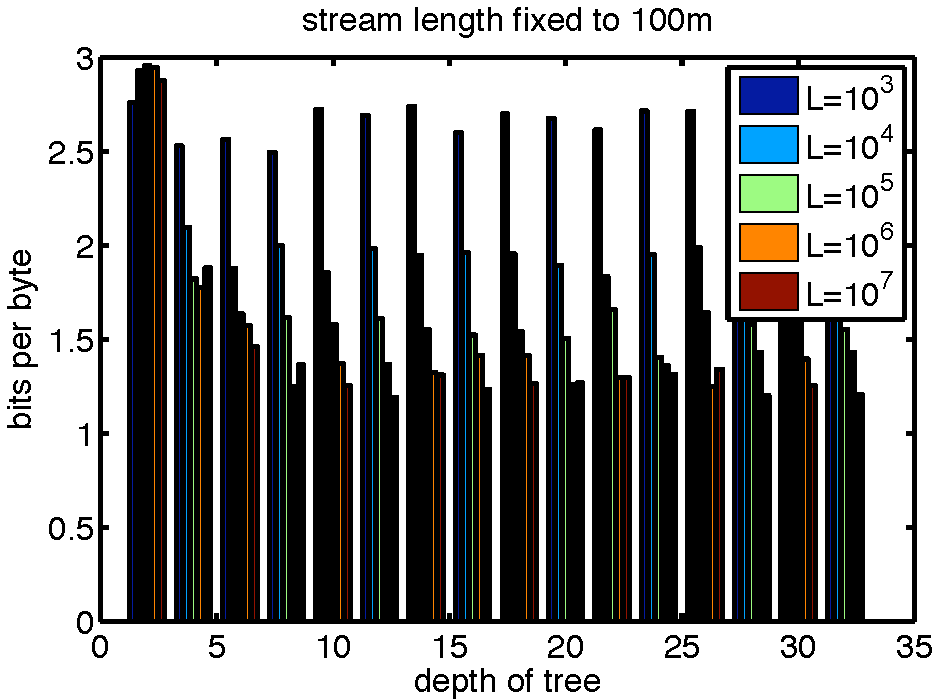
\includegraphics{figs/varying_depths.pdf}} % [clip=true, viewport= 1in 1in 9in 9in]
		\caption{Performance averaged over 10 random sections  100Mb sections of the corpus for varying fixed depths and number of allowable nodes ($L$) }
		\label{fig:varying_depths}
	\end{center} 
\end{figure*} 

%\begin{figure*}[t] 
%	\begin{center}
%		\scalebox{.6}{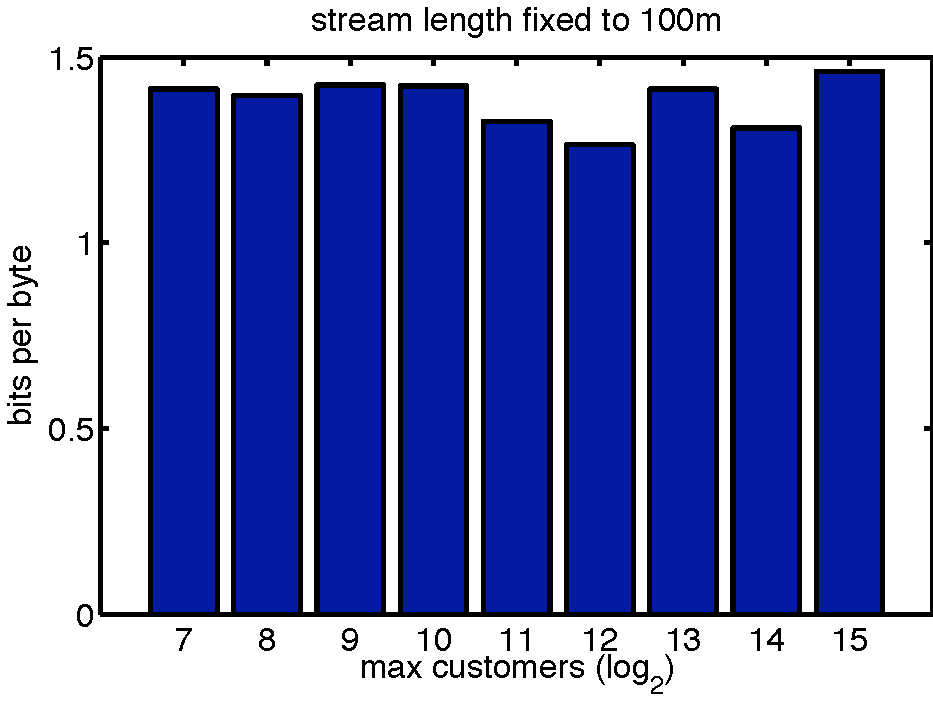
\includegraphics{figs/varying_max_customers.pdf}} % [clip=true, viewport= 1in 1in 9in 9in]
%		\caption{Performance for varying max allowable customers $k$.}
%		\label{fig: varying_max_customers}
%	\end{center} 
%\end{figure*} 

\begin{figure*}[t] 
	\begin{center}
		\scalebox{.6}{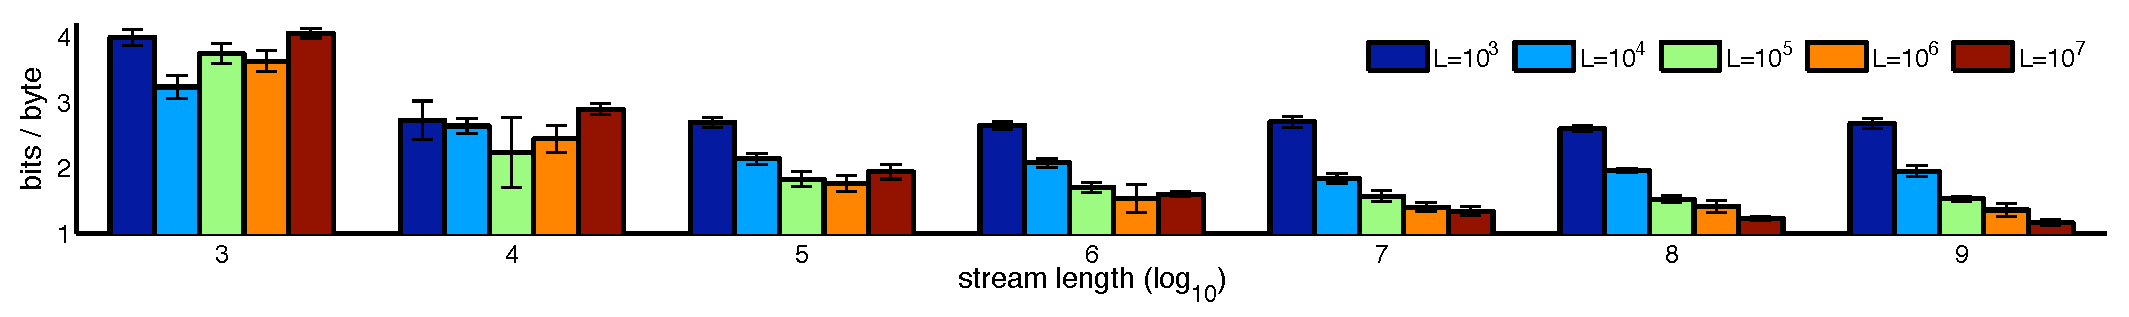
\includegraphics{figs/varying_stream_length.pdf}} % [clip=true, viewport= 1in 1in 9in 9in]
		\caption{Performance for varying stream lengths and number of allowable nodes ($L$).}
		\label{fig:varying_stream_length}
	\end{center} 
\end{figure*} 


%\begin{figure*}[t] 
%	\begin{center}
%		\scalebox{1}{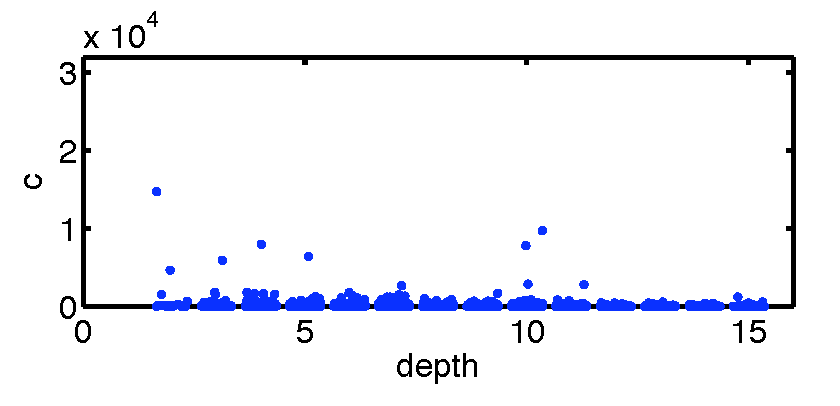
\includegraphics{figs/scatter_16.pdf}} % [clip=true, viewport= 1in 1in 9in 9in]
%		\caption{Scatter plots to explore the relationship between the depth of a node and the total count}
%		\label{fig:restaurant_plots}
%	\end{center} 
%\end{figure*} 

%\begin{figure*}[t] 
%	\begin{center}
%		\scalebox{1}{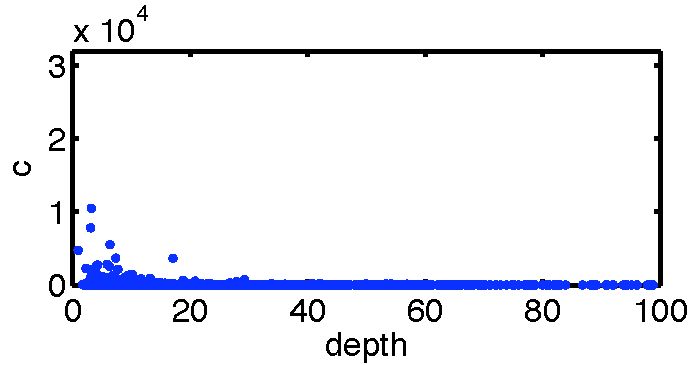
\includegraphics{figs/scatter_1024.pdf}} % [clip=true, viewport= 1in 1in 9in 9in]
%		\caption{Scatter plots to explore the relationship between the depth of a node and the total count}
%		\label{fig:restaurant_plots}
%	\end{center} 
%\end{figure*} 


%\section{Related Work}
%The sequential inference approach in PLUMP is closely related to the  \emph{prediction by
partial matching} (PPM) family of compression algorithms
\citep{cleary1984dca,moffat1990ipd,howard1993dae,cleary95unboundedlength}.
Both are based on sequentially estimating a distribution over the next symbol,
$\Prob(x_i|\xbf_{1:i-1})$ from the input seen so far and then using entropy
coding (usually arithmetic) for encoding and decoding using this distribution.
The predictive distribution $\Prob(x_i|\xbf_{1:i-1})$ in PPM is estimated by
blending estimates of the distributions over next symbols in contexts $\ubf$
which are suffixes of $\xbf_{1:i-1}$ of variable length. 
The way these distributions are blended by smoothing the counts from
related contexts of varying length resembles \eqref{eq:predictive} and the 
particle filter update algorithm. In particular, one variant, PPM-D, corresponds to a particular variant of
non-interpolated Kneser-Ney smoothing with a discount of $\frac{1}{2}$. 
Further, the  variant that uses unbounded context lengths (PPM*) also uses a suffix tree data structure that, while
quite different from the prefix tree used in the sequence memoizer, possesses
similar properties, including the $\Oh(N)$ space complexity and $\Oh(N^2)$
time complexity for prediction.

\subsection{Relation to CTW}
\begin{itemize}
    \item Infinite CTW (in the extensions paper) uses the same kind of
        compressed prefix tree (pretty sure)
    \item Each node estimates the block-joint probability using the 
        evidence of a beta-bernoulli model with params (0.5,0.5) of all 
        symbols following the context of the node
    \item The weighted probabilities are given by $P^s_w(a,b) = 0.5
        P_e^s(a,b) + 0.5 P_w^{0s}(a,b) P_w^{1s}(a,b)$.
    \item Peforms ``double mixture'' over parameters and possible models in
        the source class (tree sources)
    \item The weighted probability in each node is given by a weighting of 
    probabilities of all possible sources below the node. Coding thus is done
    using the probability computed at the root (ie. including all sources).
    \item Weighting over sources given by code length for source, e.g. more
        complex sources get less weight
\end{itemize}


% While numerous variants of the PPM scheme exists, we limit the discussion 
% here to the better-known variants PPM-A \citep{cleary1984dca}, PPM-C \citep{moffat1990ipd},
% PPM-D \citep{howard1993dae} and PPM* \citep{Cleary95unboundedlength}, 
% of which the final two are most similar to \PLUMP: PPM-D uses a similar form
% of absolute discounting and PPM* allows for unbounded-length contexts. 

% The PPM model is essentially a $k$-th order Markov model whose parameters 
% are estimated using a form of backoff smoothing. For each context with length
% $|\ubf| \leq k$ PPM estimates the distribution $\Prob(s|\ubf)$. 
% The parameters of these conditional distributions are estimated from the
% counts $c(\sbf)$ for all substrings $\sbf \in \Sigma^{k+1}$ that have been
% observed in the input seen so far. The PPM variants mainly differ in the way the
% counts are smoothed to produce the probability estimate in each context. The
% process of smoothing of the counts in PPM is typically expressed (and
% implemented) in terms of \emph{escape probabilities}.  For this, a special
% \emph{escape symbol} \texttt{esc} is included in the alphabet, and the
% distribution for each context assigns some probability to \texttt{esc}. 
% To compute the probability of the next symbol $s$ 
% given a context $\ubf$ (which we assume is always of length
% $|\ubf| = k$), PPM uses the following scheme: 
% \begin{equation}
%     \Prob(s|\ubf) = 
%     \begin{cases}
%         \hat{\Prob}(s|\ubf) & \text{if}~s \in \Sigma_{\ubf}\\
%         \hat{\Prob}(\mathtt{esc}|\ubf) \hat{\Prob}(s|\sigma(\ubf)) & \text{otherwise}
%     \end{cases}
%     \label{eq:ppmPredict}
% \end{equation}
% The probabilities $\hat{\Prob}(s|\ubf)$ and $\hat{\Prob}(\mathtt{esc}|\ubf)$
% are estimated according to the following scheme
% \begin{equation}
%     \hat{\Prob}(s|\ubf) \propto \gcount(s|\ubf)
%     \quad \quad \quad \quad
%     \hat{\Prob}(\mathtt{esc}|\ubf) \propto \gcount(\mathtt{esc}|\ubf)
%     \label{eq:ppmEstimate}
% \end{equation}
% where the normalization is with respect to all symbols in $\Sigma_{\ubf} \cup
% \{\escape\}$ which have not occurred in higher-order contexts. Because the
% symbols observed in higher-order contexts are excluded from the normalization
% this amounts to \emph{backoff} rather than \emph{interpolation} in the
% sense in which these terms are used in the language modelling community (see e.g.
% \citep{Chen:CSL99}). The definitions for
% $\gcount(\cdot|\cdot)$ are what distinguishes the various PPM variants. The 
% original PPM-A uses $\gcount(s|\ubf) = c(\ubf s)$ and $\gcount(\escape|\ubf) = 1$,
% whereas the very successful PPM-C variant uses
% $\gcount(s|\ubf) = c(\ubf s)$ and $\gcount(\escape|\ubf) = |\Sigma_{\ubf}|$.%
% \footnote{The same form of smoothing is known as Witten-Bell smoothing in the
% context of language-modelling.}
% 
% \todo{This is actually wrong!}
% PPM-D and its predecessor PPM-B are slightly different in that they use a form of absolute
% discounting and set $\gcount(s|\ubf) = c(\ubf s) - \frac{1}{2}$ and $\gcount(\escape|\ubf) =
% |\Sigma_{\ubf}|$.
% 
% PPM* uses the PPM-C scheme of probability estimation but like \PLUMP\ allows $k$ to be
% infinite, i.e. it estimates $\Prob(s|\ubf)$ for all context $\ubf$ that have
% been observed in the input. PPM* uses a suffix tree data structure that, while
% quite different from the prefix tree used in the sequence memoizer, possesses
% similar properties, including the $\Oh(N)$ space complexity and $\Oh(N^2)$
% time complexity for prediction.

% As noted in \citep{Chen:CSL99} and \citep{kneser1995ibo}, most existing
% smoothing algorithms can be written in the form 
% \begin{equation}
% \Psmooth(s|\ubf) = 
% \begin{cases}
%     \alpha(s|\ubf) & \text{if}~c(\ubf s) > 0\\
%     \gamma(\ubf) \Psmooth(s|\suffix(\ubf)) & \text{if}~ c(\ubf s)
%     = 0
% \end{cases}
% \label{eq:backoff}
% \end{equation}
% where $\alpha(s|\textbf{u})$ is the unsmoothed probability of $s$ in context
% $\ubf$ (e.g. simply $c(\ubf s)/c(\ubf)$), normalized over $s \in
% \Sigma_{\ubf}$ and $\gamma(\ubf)$ ensures normalization of $\Psmooth(s|\ubf)$.  
% Models of this form are referred to as \emph{backoff} models.
% An equivalent formulation, which is more common in the compression literature
% is in terms of \emph{escape probabilities}: For each context $\ubf$,
% $\alpha(s|\ubf)$ is modelled as a distribution over $s\in \Sigma_{\ubf} \cup
% \{\mathtt{esc}\}$ where \texttt{esc} denotes a special \emph{escape symbol}. 
% The smoothed probability for a symbol $s$ in a context
% $\ubf$ can then be written as:
% \begin{equation}
% \Psmooth(s|\ubf) = 
% \begin{cases}
%     \alpha(s|\ubf) & \text{if}~c(\ubf s) > 0\\
%     \alpha(\mathtt{esc}|\ubf) \Psmooth(s|\suffix(\ubf)) & \text{if}~ c(\ubf s)
%     = 0
% \end{cases}
% \label{eq:escape}
% \end{equation}
% An alternative to the backoff approach is linear interpolation, where the
% smoothed probability $\Psmooth(s|\ubf)$ is a convex combination of the
% unsmoothed probabilties in all contexts that are suffixes of $\ubf$: 
% \begin{equation}
%     \Psmooth(s|\ubf) = \lambda_{\ubf} \beta(s|\ubf) +
%     \lambda_{\suffix(\ubf)} \beta(s|\suffix(\ubf)) +  
%     \lambda_{\suffix(\suffix(\ubf))} \beta(s|\suffix(\suffix(\ubf))) +
%     \ldots
%     + \lambda_\epsilon \beta(s|\epsilon)
% \end{equation}
% It can easily be seen that any such \emph{interpolated
% model} can be reformulated as a backoff model by choosing 
% $\gamma(\ubf) = e_{\ubf}$ and
% $\alpha(s|\ubf) = (1-e_{\ubf})\beta(s|\ubf) + e_{\ubf}
% \Psmooth(s|\suffix(\ubf))$
% where $e_{\ubf}$ and $\lambda_{\ubf}$ are related by $\lambda_{\ubf} = (1-e_{\ubf})\prod_{\ubf' \in
% \sigma(\ubf)}e_{\ubf'}$. 
% TODO: The product above is not correct / not explained


% PPM-A and PPM-D can be expressed terms of \eqref{eq:escape} by choosing
% $\alpha(s|\suffix(\ubf)) = c(\ubf s)/(C(\ubf)+\delta)$ and
% $\alpha(\mathtt{esc}|\ubf) = \delta/(C(\ubf) + \delta)$ where $\delta$ is chosen
% to be 1 for PPM-A and $\delta=|\Sigma_s|$ for PPM-C.
% PPM-B and PPM-D can be seen as special forms of Kneser-Ney (KN)
% smoothing \citep{kneser1995ibo}. In the general form of KN smoothing
% (expressed in terms of \eqref{eq:backoff}, we have $\alpha(s|\ubf) =
% \max(c(\ubf s) - d,0)/C(\ubf)$ and $\gamma(\ubf) = \ldots $

% \begin{table}
%     \begin{center}
% \begin{tabular}{|c|c|c|}
%     \hline
%     Variant & $\alpha(s|\ubf)$ & $\alpha(\texttt{esc}|\ubf)$ \\ \hline \hline
%     A & $\frac{c(\ubf s)}{C(\ubf)+1}$ & $\frac{1}{C(\ubf) + 1}$\\
%     C & 
% \end{tabular}
% \end{center}
% \caption{Backoff interpretation of PPM variants. $C(\ubf) = \sum_{s' \in
% \Sigma_s}c(\ubf s')$}
% \end{table}


% vim: tw=78


%\section{Discussion}
%% !TEX root = main.tex
\section{Discussion}
\label{section_discussion}

Things to consider: 

1) Scaling to phrases.
2) Making the spelling correction parameterization context dependent.


\subsubsection*{Acknowledgments}
This work was supported by Google Faculty Research Award.
%This work was supported by the Gatsby Charitable Foundation and the PASCAL
%Network of Excellence.

%%% END CONTENT %%%%%%%%%%%%%%%%%%%%%%%%%%%%%%%%%%%%%%%%%%%%%%%%%%%%%%%%%%%%%%%
\renewcommand{\bibsection}{\subsubsection*{References}}
%\nocite{*}
\setlength{\bibsep}{0mm}
\bibliographystyle{apalike}
\bibliography{../uber.bib}
\end{document}
  % vim:tw=79:ts=2:sw=2:et
